% =====================================================================
%  BÁO CÁO KHOA HỌC — VietTraffic AI
%  Mô hình OCR biển số xe tự huấn luyện (train — SVTRv2-inspired CTC)
% ---------------------------------------------------------------------
%  Biên dịch: pdfLaTeX (khuyến nghị Overleaf, biên dịch 2 lần để cập
%  nhật mục lục). Hỗ trợ tiếng Việt qua babel + fontenc T5.
%  Nếu dùng XeLaTeX/LuaLaTeX, có thể thay phần font bằng fontspec.
% =====================================================================
\documentclass[12pt,a4paper]{report}

% --- Hỗ trợ tiếng Việt cho cả pdfLaTeX (Overleaf) lẫn XeLaTeX/LuaLaTeX ---
\usepackage{iftex}
\ifPDFTeX
  \usepackage[utf8]{inputenc}
  \usepackage[T5]{fontenc}
  \usepackage[vietnamese]{babel}
  \usepackage{mathptmx} % Font kiểu Times New Roman cho pdfLaTeX
\else
  \usepackage{fontspec}
  \usepackage{polyglossia}
  \setmainlanguage{vietnamese}
  % Font kiểu Times New Roman (Unicode, hỗ trợ tiếng Việt)
  \IfFontExistsTF{Times New Roman}{\setmainfont{Times New Roman}}{%
    \IfFontExistsTF{Liberation Serif}{\setmainfont{Liberation Serif}}{%
      \IfFontExistsTF{TeX Gyre Termes}{\setmainfont{TeX Gyre Termes}}{%
        \setmainfont{DejaVu Serif}}}}
\fi

\usepackage[a4paper,margin=2.5cm]{geometry}
\usepackage{amsmath,amssymb}
\usepackage{booktabs}
\usepackage{array}
\usepackage{longtable}
\usepackage{graphicx}
\usepackage{xcolor}
\usepackage{enumitem}
\usepackage{caption}
\usepackage{float}
\usepackage{tikz}
\usetikzlibrary{shapes.geometric,arrows.meta,positioning}
\usepackage[hidelinks]{hyperref}

% --- Màu dùng cho hộp ghi chú ---
\definecolor{primary}{RGB}{20,70,120}
\definecolor{accent}{RGB}{200,80,30}
\definecolor{lightgray}{RGB}{240,240,240}

% Số trang ở giữa chân trang (giống file mẫu), không header màu
\pagestyle{plain}

% --- Hộp ghi chú ---
\newcommand{\note}[1]{%
  \begin{center}
  \fcolorbox{primary}{lightgray}{%
    \parbox{0.93\linewidth}{\small #1}}
  \end{center}}

% --- Bao chèn ảnh an toàn: chỉ chèn nếu file tồn tại ---
\newcommand{\safeimage}[3]{%
  \IfFileExists{#1}{%
    \begin{figure}[H]\centering
      \includegraphics[width=#2\linewidth]{#1}
      \caption{#3}
    \end{figure}}{%
    \begin{figure}[H]\centering
      \fcolorbox{gray}{lightgray}{\parbox{#2\linewidth}{\centering\vspace{1.2cm}
      \textit{[Hình minh hoạ: #3]}\\ \small\texttt{\detokenize{#1}}\vspace{1.2cm}}}
      \caption{#3}
    \end{figure}}}

\renewcommand{\arraystretch}{1.25}

% =====================================================================
\begin{document}

% ----------------------------- TRANG BÌA -----------------------------
\begin{titlepage}
\thispagestyle{empty}
\centering
% Khung viền đôi quanh trang bìa
\setlength{\fboxrule}{1.2pt}\setlength{\fboxsep}{0pt}%
\fbox{\setlength{\fboxrule}{0.5pt}\setlength{\fboxsep}{10pt}\fbox{%
\begin{minipage}[c][0.93\textheight][c]{0.9\textwidth}
\centering
{\large\bfseries TRƯỜNG ĐẠI HỌC XÂY DỰNG HÀ NỘI}\\[3pt]
{\large\bfseries KHOA CÔNG NGHỆ THÔNG TIN}\\[24pt]

\IfFileExists{docs/images/logo_truong.png}{%
  
\includegraphics[width=3.2cm]{docs/images/logo_truong.png}}{}

\vspace{24pt}
{\large\bfseries BÁO CÁO ĐỒ ÁN MÔN HỌC}\\[4pt]
{\Large\bfseries THỊ GIÁC MÁY TÍNH}

\vspace{14pt}
\rule{0.6\linewidth}{0.4pt}

\vspace{12pt}
{\itshape Đề tài:}

\vspace{12pt}
{\LARGE\bfseries Hệ thống nhận diện biển số\\[4pt]
ứng dụng cho phát hiện phương tiện\\[4pt]
và đi sai làn}

\vspace{12pt}
\rule{0.6\linewidth}{0.4pt}

\vspace{40pt}
\begin{minipage}{0.82\linewidth}
\begin{tabular}{rl}
\textbf{Sinh viên thực hiện:} & Hoàng Thị Hoạt \quad 0294068 \\
 & Đỗ Công Trí \quad\;\; 0214268 \\
 & Nguyễn Đức Mạnh \;\; 0210668 \\[3pt]
\textbf{Lớp:} & 68CS2 \\[3pt]
\textbf{Giảng viên hướng dẫn:} & GV. Nguyễn Đình Quý \\
\end{tabular}
\end{minipage}

\vfill
{Hà Nội, năm 2026}
\end{minipage}}}
\end{titlepage}

% --------------------------- LỜI MỞ ĐẦU ---------------------------
\pagenumbering{arabic}
\chapter*{Lời mở đầu}
\addcontentsline{toc}{chapter}{Lời mở đầu}
\thispagestyle{plain}

Lời đầu tiên, nhóm thực hiện xin bày tỏ lòng biết ơn chân thành tới thầy Nguyễn Đình Quý, giảng viên hướng dẫn.

Báo cáo trình bày quá trình xây dựng một hệ thống thị giác máy tính giám sát giao thông tại nút giao theo một luồng xử lý thống nhất, từ phát hiện và bám vết phương tiện, phân tích hành vi đi sai làn, cho đến đọc biển số của xe vi phạm nhằm định danh phục vụ công tác xử phạt. Trong toàn bộ hệ thống, mô-đun nhận dạng ký tự biển số là khâu định danh có tính quyết định và cũng là phần được nhóm đầu tư chuyên sâu nhất. Khi trình bày kết quả, nhóm cố gắng ghi rõ điều kiện đo của từng con số và nêu cả mặt làm được lẫn phần còn hạn chế, để báo cáo bám sát đúng những gì sản phẩm thực sự đạt được.

Nhóm xin cam đoan đồ án là công trình do nhóm tự nghiên cứu và xây dựng dưới sự hướng dẫn của thầy Nguyễn Đình Quý. Toàn bộ mã nguồn, thiết kế và nội dung báo cáo do nhóm trực tiếp thực hiện; các tài liệu, thư viện và công nghệ của bên thứ ba đều được trích dẫn, ghi nhận đầy đủ. Các số liệu và kết quả kiểm thử nêu trong báo cáo là trung thực, phản ánh đúng sản phẩm đã hiện thực. Mặc dù đã hết sức cố gắng, báo cáo khó tránh khỏi những thiếu sót; nhóm rất mong nhận được các ý kiến đóng góp của quý thầy cô để sản phẩm ngày càng hoàn thiện hơn.

\vspace{1.2em}
\begin{flushright}
\textit{Nhóm sinh viên thực hiện}\\[3pt]
Hoàng Thị Hoạt \quad Đỗ Công Trí \quad Nguyễn Đức Mạnh
\end{flushright}

% ----------------------------- TÓM TẮT -----------------------------
\chapter*{Tóm tắt}
\addcontentsline{toc}{chapter}{Tóm tắt}
\thispagestyle{plain}

Báo cáo tập trung vào việc xây dựng mô-đun nhận dạng ký tự biển số xe (OCR) cho một hệ thống giám sát giao thông, trong đó trọng tâm là một mô hình nhận dạng tự huấn luyện, gọi tắt là \emph{train}. Mô hình được thiết kế theo kiến trúc lấy cảm hứng từ SVTRv2, kết hợp trích đặc trưng cục bộ bằng mạng tích chập, bộ mã hoá Transformer để học ngữ cảnh chuỗi, và cơ chế huấn luyện đa nhiệm với một nhánh phụ dự đoán sự hiện diện ký tự. Toàn bộ mô hình được huấn luyện hoàn toàn từ đầu trên GPU Kaggle T4$\times$2, chỉ sử dụng tập dữ liệu được cung cấp và không dùng bất kỳ trọng số tiền huấn luyện nào.

Nhằm phản ánh đúng năng lực của mô hình, báo cáo tách bạch hai mức kết quả: kết quả thô của riêng mô hình và kết quả của toàn bộ pipeline sau khi áp dụng bộ giải mã ràng buộc theo định dạng biển số Việt Nam. Trên tập kiểm thử gồm 1.219 ảnh thực tế, toàn pipeline đạt 93,06\% độ chính xác ký tự và 75,39\% độ chính xác toàn biển ở tốc độ thời gian thực, trong khi năng lực nhận dạng thô của mô hình đo trên tập kiểm chuẩn đạt 51,31\%. Báo cáo phân tích nguyên nhân của khoảng cách này, so sánh công bằng với các hướng cải tiến dựa trên kiến trúc CRNN, đồng thời chỉ ra cả điểm mạnh lẫn hạn chế của mô hình để làm cơ sở cho hướng phát triển tiếp theo.

\vspace{0.6em}
\noindent\textbf{Từ khoá:} nhận dạng biển số, OCR, CTC, SVTRv2, huấn luyện từ đầu, giám sát giao thông.

\tableofcontents

% =====================================================================
\chapter{Giới thiệu}

\section{Đặt vấn đề}
Giao thông tại các đô thị lớn của Việt Nam có mật độ phương tiện rất cao, nhất là ở những nút giao ngã tư vào giờ cao điểm. Ở các vị trí này, hành vi đi sai làn diễn ra khá phổ biến: xe đang ở làn bắt buộc rẽ trái nhưng lại đi thẳng, hoặc ngược lại. Trong khi đó, phần lớn camera lắp tại ngã tư hiện nay mới chỉ dừng ở mức ghi hình, còn việc theo dõi và phát hiện vi phạm vẫn do con người thực hiện thủ công. Cách làm này tốn nhiều nhân lực, khó duy trì liên tục trong thời gian dài, dễ bỏ sót và phụ thuộc vào cảm tính của người quan sát.

Từ thực tế đó, đồ án đặt ra nhu cầu xây dựng một hệ thống có khả năng phân tích trực tiếp luồng video tại ngã tư để phát hiện hành vi vi phạm, đồng thời nhận diện được biển số của phương tiện gây ra vi phạm. Trong đó, việc đọc biển số không phải một chức năng tách rời mà chính là khâu định danh phương tiện: nếu không xác định được biển số thì việc phát hiện vi phạm cũng khó dẫn tới một hồ sơ xử phạt có giá trị. Vì lý do đó, trong toàn bộ hệ thống, mô-đun nhận dạng ký tự biển số (OCR) được xem là thành phần then chốt và là trọng tâm kỹ thuật của báo cáo này.

Bài toán nhận dạng biển số ở điều kiện thực tế khó hơn nhiều so với khi đọc trên ảnh quét sạch. Ảnh thu từ camera giao thông thường bị mờ do xe di chuyển nhanh, rung khi có phương tiện nặng đi qua, thiếu sáng vào ban đêm, hoặc biển bị bám bụi và che khuất một phần. Biển số Việt Nam cũng đa dạng về định dạng (biển dài của ô tô, biển vuông hai dòng của xe máy) và màu nền (trắng, vàng, xanh, đỏ), kèm theo ký tự đặc thù như chữ \texttt{Đ} dễ bị nhầm khi ảnh nhiễu. Những yếu tố này khiến độ chính xác ``đọc đúng toàn bộ biển'' trở thành thước đo khắt khe, bởi chỉ cần sai một ký tự là cả biển số bị coi như sai.

\section{Mục tiêu và phạm vi}
Mục tiêu chính của đồ án là xây dựng một pipeline hoàn chỉnh, liền mạch từ đầu vào là đoạn video quay tại ngã tư cho đến đầu ra là hồ sơ vi phạm gồm loại lỗi, biển số của xe vi phạm và ảnh bằng chứng kèm theo. Trong đó, nhóm tập trung phát triển mô-đun OCR cho biển số Việt Nam, thử nhiều phương pháp rồi đánh giá để chọn phương án phù hợp, và xây dựng một bản demo chạy được trên dữ liệu thực.

Riêng với mô hình OCR, nhóm tự đặt ra ba ràng buộc để bài toán vừa khả thi vừa cho kết quả đáng tin và có thể tái lập. Thứ nhất về phần cứng, toàn bộ quá trình huấn luyện chỉ dùng GPU miễn phí Kaggle T4$\times$2. Thứ hai về dữ liệu, mô hình chỉ học trên tập \texttt{ocr\_dataset} được cung cấp, không bổ sung nhãn từ nguồn bên ngoài. Thứ ba về phương pháp, mô hình trọng tâm (được gọi là \emph{train} trong báo cáo) được huấn luyện hoàn toàn từ đầu, tức khởi tạo trọng số ngẫu nhiên, không dùng mô hình tiền huấn luyện và không tinh chỉnh từ các bộ nhận dạng chữ lớn có sẵn.

Về phạm vi, đồ án giới hạn ở dữ liệu quay tại một ngã tư cố định và chỉ xét loại vi phạm đi sai làn đường, kèm việc nhận diện biển số của phương tiện vi phạm. Các lỗi khác như vượt đèn đỏ hay chạy quá tốc độ nằm ngoài phạm vi và chỉ được nêu như hướng phát triển trong tương lai.

\section{Tổng quan kiến trúc hệ thống}
Hệ thống được tổ chức theo một luồng xử lý thống nhất gồm các khối nối tiếp, mô tả ở Hình~\ref{fig:pipeline}. Khối đầu tiên nhận luồng video và thực hiện phát hiện cùng bám vết phương tiện: bộ phát hiện YOLOv8m định vị các xe trong khung hình, còn thuật toán bám vết ByteTrack gán cho mỗi xe một mã định danh ổn định qua nhiều khung. Để giảm tải, hệ thống chỉ giám sát các xe nằm trong vùng quan tâm (ROI) được xác định theo tỉ lệ toạ độ, thay vì toàn bộ khung hình. Khối thứ hai phân tích hành vi đi sai làn: mặt đường được mô tả bằng các vùng đa giác (gồm các làn và vùng hướng), và bằng cách đối chiếu quỹ đạo của từng xe với chuỗi vùng mà nó đi qua, hệ thống kết luận xe có vi phạm hay không theo các trường hợp luật được định nghĩa trước trên cơ sở Nghị định 168/2024/NĐ-CP.

Khối thứ ba chỉ xử lý những xe đã bị kết luận vi phạm. Một bộ phát hiện biển số riêng (mô hình YOLO chuyên biệt) cắt vùng biển số từ ảnh xe với phần lề mở rộng để tránh mất ký tự ở mép; trong số nhiều khung hình của cùng một xe, hệ thống chấm điểm độ nét (dựa trên phương sai Laplacian) và một số tiêu chí khác để chọn ra ảnh biển số rõ nhất đưa vào nhận dạng. Khối thứ tư là mô-đun OCR đọc chuỗi ký tự từ ảnh biển số đã chọn; kết quả thô tiếp tục đi qua khâu hậu xử lý ràng buộc theo định dạng biển số Việt Nam để chuẩn hoá. Cuối cùng, khối thứ năm tổng hợp kết quả, lưu vào cơ sở dữ liệu (SQLite) thông qua một dịch vụ nền viết bằng FastAPI và hiển thị trên giao diện web phục vụ tra cứu, quản trị bằng chứng vi phạm.

\begin{figure}[H]
\centering
\begin{tikzpicture}[
  node distance=0.45cm,
  blk/.style={draw,rounded corners,align=center,text width=2.15cm,minimum height=1.7cm,font=\scriptsize},
  hl/.style={blk,fill=primary!15,line width=1.1pt},
  arr/.style={-{Latex[length=2mm]},thick}]
  \node[blk] (a) {Phát hiện \& bám vết\\(YOLOv8m + ByteTrack)};
  \node[blk,right=of a] (b) {Phân tích sai làn\\(5 vùng đa giác)};
  \node[blk,right=of b] (c) {Phát hiện biển số\\(YOLO + chọn khung nét)};
  \node[hl,right=of c] (d) {Nhận dạng OCR\\+ hậu xử lý luật};
  \node[blk,right=of d] (e) {Lưu trữ \& giao diện\\(FastAPI/SQLite)};
  \draw[arr] (a)--(b); \draw[arr] (b)--(c); \draw[arr] (c)--(d); \draw[arr] (d)--(e);
\end{tikzpicture}
\caption{Luồng xử lý thống nhất của hệ thống. Khối nhận dạng OCR (tô đậm) là trọng tâm kỹ thuật của báo cáo.}
\label{fig:pipeline}
\end{figure}

Hai khối nặng nhất (phát hiện biển số và OCR) chỉ chạy khi cần, nhờ đó hệ thống có ba chế độ vận hành: chỉ giám sát biển số (luôn đọc biển mọi xe), chỉ giám sát sai làn (tắt phần biển số và OCR để tiết kiệm tài nguyên), và phạt nguội tích hợp (chỉ đọc biển khi phát hiện xe vi phạm).

Trong kiến trúc này, các khối phát hiện, bám vết, phân tích làn, lưu trữ và giao diện chỉ được trình bày ở mức tổng quan; trọng tâm nhóm đi sâu là khối nhận dạng ký tự biển số.

% =====================================================================
\chapter{Cơ sở lý thuyết}

\section{Nhận dạng ký tự biển số như một bài toán đọc chuỗi}
Đọc biển số thuộc nhóm nhận dạng văn bản trong ảnh (Scene Text Recognition). Cách cổ điển tách rời và phân loại từng ký tự, nhưng việc cắt ký tự rất nhạy với nhiễu và mờ nên dễ sai dây chuyền. Báo cáo đi theo hướng hiện đại: xem cả biển số là một chuỗi và để mạng tự đọc mà không cần cắt ký tự, vì ảnh biển thực tế thường không đủ rõ để phân đoạn đáng tin cậy.

Khi coi biển số là chuỗi, đầu vào là một ảnh đã được chuẩn hoá kích thước, còn đầu ra là một dãy ký tự có độ dài thay đổi (biển Việt Nam thường dài khoảng tám đến mười một ký tự). Khó khăn cốt lõi nằm ở chỗ ta chỉ có nhãn là chuỗi văn bản, chứ không biết mỗi ký tự nằm ở cột nào của ảnh. Đây chính là vấn đề mà hàm mất mát CTC được thiết kế để giải quyết.

\section{Hàm mất mát CTC cho chuỗi không căn chỉnh}
Connectionist Temporal Classification (CTC), do Graves và cộng sự đề xuất năm 2006, cho phép huấn luyện một mô hình đọc chuỗi mà không cần nhãn vị trí của từng ký tự. Ý tưởng là mô hình xuất ra một dãy phân phối xác suất theo trục thời gian, ở đây là theo chiều ngang của ảnh, với độ dài $T$ lớn hơn nhiều so với số ký tự thật. Bảng ký tự được bổ sung một ký hiệu trống (\emph{blank}). Mỗi đường đi $\pi$ độ dài $T$ trên bảng ký tự mở rộng được gọi là một cách căn chỉnh; phép thu gọn $\mathcal{B}$ sẽ bỏ các ký tự lặp liên tiếp rồi bỏ \emph{blank} để thu về chuỗi cuối.

Xác suất của một nhãn $\mathbf{y}$ được tính bằng tổng xác suất của mọi cách căn chỉnh thu gọn về $\mathbf{y}$, và hàm mất mát là log-âm của xác suất đó:
\begin{equation}
p(\mathbf{y}\mid \mathbf{x}) = \sum_{\pi \in \mathcal{B}^{-1}(\mathbf{y})} \prod_{t=1}^{T} p(\pi_t \mid \mathbf{x}),
\qquad
\mathcal{L}_{\text{CTC}} = -\log p(\mathbf{y}\mid \mathbf{x}).
\end{equation}
Tổng này có thể tính hiệu quả bằng quy hoạch động tiến--lùi (forward--backward). Khi suy luận, cách giải mã đơn giản nhất là tham lam (greedy): mỗi bước chọn ký tự có xác suất cao nhất rồi áp phép thu gọn $\mathcal{B}$.

CTC có nhiều ưu điểm cho bài toán biển số: không cần nhãn vị trí, xử lý được biển dài ngắn khác nhau, và nhờ ký hiệu \emph{blank} nên tách được hai ký tự giống nhau liền kề. Hạn chế là CTC giả định các bước thời gian độc lập có điều kiện, nên không tự nắm các ràng buộc kiểu ``ngôn ngữ'' giữa các ký tự; vì thế cần một bộ trích đặc trưng đủ mạnh phía trước và một bước hậu xử lý theo luật định dạng phía sau.

\section{Trích đặc trưng thị giác: tích chập và tự chú ý}
Trước hết cần biến ảnh thành một dãy đặc trưng. Mạng tích chập (CNN) phù hợp cho việc này: nhờ tính cục bộ, các lớp tích chập học tốt đặc trưng nét chữ như cạnh, góc và đường cong. Hầu hết bộ nhận dạng chuỗi đều bắt đầu bằng một thân CNN để giảm độ phân giải và cô đọng đặc trưng.

Sau khi có đặc trưng cục bộ, mô hình cần học quan hệ giữa các vị trí trong chuỗi. Kiến trúc CRNN kinh điển của Shi và cộng sự (2015) dùng mạng hồi tiếp hai chiều (BiLSTM) cho mục đích này. Tuy nhiên, BiLSTM phải tính tuần tự qua từng bước thời gian nên hạn chế khả năng song song trên GPU, và mối phụ thuộc tầm xa có thể bị suy yếu theo khoảng cách. Cơ chế tự chú ý (self-attention) trong kiến trúc Transformer (Vaswani và cộng sự, 2017) khắc phục được cả hai điểm: mọi vị trí trong chuỗi tương tác trực tiếp với nhau, vừa tận dụng tốt tính toán song song, vừa mô hình hoá quan hệ tầm xa một cách tường minh. Họ mô hình SVTR và phiên bản SVTRv2 phát triển ý tưởng kết hợp ``trộn'' đặc trưng ở hai cấp: trộn cục bộ bằng các khối kiểu tích chập để nắm nét chữ, và trộn toàn cục bằng tự chú ý để nắm bố cục và thứ tự ký tự. Mô hình train trong báo cáo được thiết kế theo tinh thần này.

Dù vậy, lợi thế của Transformer không phải là tuyệt đối. Với chuỗi ngắn chỉ vài ký tự như biển số, ưu thế về quan hệ tầm xa không lớn, trong khi tự chú ý lại cần nhiều dữ liệu hơn để học tốt khi huấn luyện từ đầu. Đây là một đánh đổi có rủi ro.

\section{Học đa nhiệm và giám sát phụ trợ}
Một kỹ thuật thường được dùng để giúp mô hình hội tụ tốt hơn là gắn thêm một nhánh đầu ra phụ trong lúc huấn luyện. Bên cạnh nhánh chính dự đoán chuỗi bằng CTC, mô hình có thể có một nhánh phụ dự đoán tập các ký tự xuất hiện trong ảnh mà không quan tâm thứ tự, huấn luyện bằng hàm Binary Cross-Entropy. Hai nhánh được tối ưu đồng thời theo tổng có trọng số
\begin{equation}
\mathcal{L} = \mathcal{L}_{\text{CTC}} + \lambda_{\text{sem}}\,\mathcal{L}_{\text{BCE}}.
\end{equation}
Nhánh phụ đóng vai trò một dạng giám sát phụ trợ (auxiliary supervision): nó cung cấp thêm tín hiệu học cho phần thân CNN ngay từ giai đoạn đầu, khi tín hiệu từ CTC còn yếu do các cách căn chỉnh chưa ổn định, qua đó giúp backbone sớm học được đặc trưng phân biệt ký tự. Đây là kỹ thuật khá phổ biến và sẽ được áp dụng trong train với trọng số nhỏ.

\section{Phát hiện và định vị biển số}
Trước khi đọc được biển, hệ thống phải tìm và cắt vùng biển, đây là bài toán phát hiện đối tượng. Các bộ phát hiện một giai đoạn như họ YOLO làm việc này trong một lượt truyền thẳng: ảnh được chia thành lưới ô, mỗi ô dự đoán hộp bao, điểm objectness và lớp đối tượng, nên đạt tốc độ cao phù hợp với xử lý thời gian thực. Hai khái niệm đi kèm là tỉ số giao trên hợp (IoU) để đo mức trùng khớp giữa hai hộp, và bước khử trùng (NMS) để mỗi vật chỉ còn một dự đoán. Trong hệ thống, việc tìm biển được tách hai bước (phát hiện xe rồi mới dò biển trong vùng xe) và chọn khung biển rõ nhất theo độ nét; chi tiết triển khai nằm ở chương về khối phát hiện.

\section{Bám vết phương tiện và phát hiện đi sai làn}
Để phân tích hành vi, mỗi xe cần được theo dõi liên tục, tức gán một mã định danh ổn định qua các khung. Đây là bài toán bám vết đa đối tượng theo mô hình ``bám vết dựa trên phát hiện''; một phương pháp tiêu biểu là ByteTrack, dùng bộ lọc Kalman để dự đoán chuyển động và ghép vết theo IoU, cho ra quỹ đạo từng xe. Trên quỹ đạo đó, việc xác định đi sai làn được quy về bài toán hình học: mỗi làn là một đa giác, dùng kiểm tra điểm trong đa giác để biết xe ở làn nào, rồi đối chiếu chuỗi vùng đã đi qua với một bộ luật để kết luận. Cách dựa trên luật dễ giải thích và cho bằng chứng rõ ràng; chi tiết nằm ở chương về khối phát hiện sai làn.

\section{Các độ đo đánh giá}
Để đánh giá khách quan, báo cáo sử dụng một số độ đo chuẩn cho bài toán nhận dạng chuỗi. Nền tảng là khoảng cách chỉnh sửa Levenshtein, ký hiệu $d_\text{lev}(\hat{y}, y)$, là số thao tác chèn, xoá hoặc thay thế tối thiểu để biến chuỗi dự đoán $\hat{y}$ thành nhãn $y$.

Độ chính xác ký tự (Character Accuracy) và tỉ lệ lỗi ký tự (CER) được tính trên toàn tập:
\begin{equation}
\text{CharAcc} = 1 - \frac{\sum_i d_\text{lev}(\hat{y}_i, y_i)}{\sum_i \max(|\hat{y}_i|, |y_i|)},
\qquad
\text{CER} = 1 - \text{CharAcc}.
\end{equation}
Độ chính xác toàn biển (Full Plate Accuracy, hay Sequence Accuracy) là độ đo khắt khe hơn, chỉ tính một biển là đúng khi mọi ký tự đều khớp sau chuẩn hoá:
\begin{equation}
\text{PlateAcc} = \frac{1}{N}\sum_{i=1}^{N} \mathbf{1}\!\left[\hat{y}_i = y_i\right].
\end{equation}
Ngoài ra, khoảng cách chỉnh sửa trung bình giúp định lượng mức độ sai (sai một ký tự khác hẳn sai nhiều ký tự), còn về vận hành, báo cáo theo dõi thời gian suy luận trung bình, trung vị, phân vị 95 (P95) và thông lượng (số ảnh xử lý mỗi giây) để đánh giá khả năng chạy thời gian thực. Khoảng cách giữa CharAcc cao và PlateAcc thấp hơn cho thấy phần lớn lỗi chỉ là sai lệch một vài ký tự; nhưng vì tiêu chí toàn biển rất khắt khe nên chỉ cần một ký tự sai là cả biển bị tính sai.

% =====================================================================
\chapter{Dữ liệu và tiền xử lý}

\section{Thống kê dữ liệu thực tế}
Dữ liệu thật được tách theo ba tập như Bảng~\ref{tab:data}. Bảng chữ cái nhận dạng (charset) gồm 36 ký tự: các chữ số \texttt{0--9}, chữ cái \texttt{A--Z} (loại \texttt{W}), và ký tự đặc thù tiếng Việt \texttt{Đ}.

\begin{table}[H]
\centering
\caption{Phân chia tập dữ liệu thật (\texttt{ocr\_dataset}).}
\label{tab:data}
\begin{tabular}{lcc}
\toprule
\textbf{Tập} & \textbf{Số ảnh} & \textbf{Vai trò} \\
\midrule
Train & 9.752 & Huấn luyện tham số mô hình \\
Validation & 1.219 & Chọn checkpoint, theo dõi hội tụ \\
Test & 1.219 & Đánh giá cuối cùng, độc lập \\
\midrule
\textbf{Tổng} & \textbf{12.190} & \\
\bottomrule
\end{tabular}
\end{table}

\section{Sửa lỗi mã hoá nhãn (Mojibake)}
Do dữ liệu thu từ nhiều nguồn, nhãn thường lỗi mã hoá ký tự \texttt{Đ/đ} tiếng Việt. Pipeline tiền xử lý tự động ánh xạ lại (\texttt{Ä }, \texttt{Ð} $\rightarrow$ \texttt{Đ}; \texttt{Ä'} $\rightarrow$ \texttt{đ}), đồng bộ về chữ in hoa và loại khoảng trắng thừa, sau đó chuyển nhãn văn bản thô sang định dạng CSV chuẩn hoá.

\section{Sinh dữ liệu tổng hợp và tăng cường}
Để bù dữ liệu hiếm (biển đỏ quân đội, biển xanh công vụ, xe điện) và tăng độ bền với nhiễu, train tích hợp bộ sinh biển số tổng hợp với \texttt{synthetic\_ratio = 5} (mỗi ảnh thật kèm 5 ảnh tổng hợp, nâng quy mô huấn luyện ảo lên $\approx 58.512$ mẫu). Chuỗi tăng cường gồm: xoay $\pm3^\circ$ đến $\pm15^\circ$, biến đổi phối cảnh QUAD, hạ độ phân giải rồi nội suy lại (mô phỏng biển ở xa), motion blur + Gaussian blur, và nén JPEG chất lượng rất thấp (10--35) để giả lập luồng video nén. Ngoài ra, train dùng \emph{multi-size bucketing} (40$\times$160, 48$\times$192, 56$\times$224) để giảm méo ký tự khi đổi tỷ lệ khung hình.

Chiến lược sinh dữ liệu mạnh là hợp lý khi dữ liệu thật ít (chỉ khoảng 9.700 ảnh). Tuy nhiên, tỉ lệ \texttt{synthetic\_ratio = 5} là khá cao: nếu phân phối ảnh tổng hợp lệch khỏi ảnh thật, mô hình có nguy cơ ``trôi'' về đặc trưng tổng hợp (synthetic drift). Đây là một yếu tố cần kiểm soát và sẽ được bàn thêm ở phần điểm yếu.

% =====================================================================
\chapter{Kiến trúc mô hình nhận dạng (trái tim hệ thống)}

Khối nhận dạng ký tự biển số là trái tim của hệ thống: mọi khâu phía trước đều nhằm đưa một ảnh biển số tới đây, và giá trị pháp lý của hồ sơ vi phạm phụ thuộc vào việc khối này đọc đúng hay sai, bởi chỉ sai một ký tự là cả hồ sơ mất hiệu lực. Đây cũng là thành phần nhóm đầu tư nhất. Chương này trình bày chi tiết kiến trúc của mô hình.

\section{Tổng quan kiến trúc}
Mô hình \emph{train} được xây dựng theo tinh thần của họ SVTRv2: dùng một thân chung gồm thân tích chập và khối trộn cục bộ để rút đặc trưng, sau đó \emph{tách thành hai nhánh song song} cùng được huấn luyện một lúc. Nhánh thứ nhất, gọi là \textbf{nhánh tuần tự}, đọc biển số như một chuỗi ký tự bằng Transformer và CTC; đây là nhánh chính, cũng là nhánh duy nhất được dùng khi suy luận. Nhánh thứ hai, gọi là \textbf{nhánh ngữ nghĩa}, dự đoán \emph{tập ký tự xuất hiện} trong ảnh mà không quan tâm thứ tự; nhánh này chỉ dùng trong lúc huấn luyện như một tín hiệu giám sát phụ. Điểm cần nhấn mạnh là hai nhánh tách ra \emph{ngay sau thân chung}: nhánh tuần tự gộp đặc trưng theo chiều cao để tạo chuỗi, còn nhánh ngữ nghĩa gộp toàn bộ đặc trưng bằng Global Average Pooling thành một vector. Hình~\ref{fig:arch} mô tả toàn bộ đường đi này.

\begin{figure}[H]
\centering
\begin{tikzpicture}[
  font=\small,
  box/.style={draw,thin,fill=white,align=center,text width=7.0cm,minimum height=0.8cm,inner sep=3pt},
  sb/.style={draw,thin,fill=white,align=center,text width=4.4cm,minimum height=0.8cm,inner sep=3pt},
  lab/.style={font=\scriptsize\itshape},
  arr/.style={-{Latex[length=2mm]},semithick},
  node distance=5mm]
  \node[box] (in) {Ảnh biển số đầu vào ($48\times192\times3$)};
  \node[box,below=of in] (stem) {CNN Stem ($3\times$ Conv $3\times3$ + BN + GeLU + Pool)};
  \node[box,below=of stem] (lmb) {Local Mixing Block (Depthwise Separable Conv + FFN)};
  % hai nhánh
  \node[sb,below=12mm of lmb,xshift=-3.5cm] (seq) {\textit{Nhánh tuần tự}\\Gộp theo chiều cao $\rightarrow$ chuỗi};
  \node[sb,below=12mm of lmb,xshift=3.5cm] (gap) {\textit{Nhánh ngữ nghĩa}\\Global Average Pooling $\rightarrow$ vector};
  \node[sb,below=of seq] (pe) {Cộng Positional Encoding};
  \node[sb,below=of pe] (tr) {Transformer Encoder (8 lớp, 8 heads)};
  \node[sb,below=of tr] (ctc) {CTC Head (Linear $\rightarrow$ Softmax)};
  \node[below=5mm of ctc,font=\footnotesize,align=center] (octc) {Chuỗi ký tự\\ $\mathcal{L}_{\text{CTC}}$};
  \node[sb,below=of gap] (sem) {Semantic Head (Sigmoid)};
  \node[below=of sem,font=\footnotesize,align=center] (osem) {Tập ký tự có mặt\\ $\mathcal{L}_{\text{BCE}}$};
  \draw[arr] (in)--(stem); \draw[arr] (stem)--(lmb);
  \draw[arr] (lmb.south)--(seq.north);
  \draw[arr] (lmb.south)--(gap.north);
  \draw[arr] (seq)--(pe); \draw[arr] (pe)--(tr); \draw[arr] (tr)--(ctc); \draw[arr] (ctc)--(octc);
  \draw[arr] (gap)--(sem); \draw[arr] (sem)--(osem);
\end{tikzpicture}
\caption{Kiến trúc mô hình nhận dạng. Sau thân chung (CNN Stem + Local Mixing), dữ liệu tách thành nhánh tuần tự (đọc chuỗi bằng Transformer + CTC) và nhánh ngữ nghĩa (Global Average Pooling + Semantic Head). Khi suy luận chỉ dùng nhánh tuần tự.}
\label{fig:arch}
\end{figure}

\section{Chuẩn hoá đầu vào}
Mỗi ảnh biển số được đưa về kích thước cố định $48\times192$ điểm ảnh, ba kênh màu, rồi chuẩn hoá giá trị điểm ảnh trước khi vào mạng. Bảng ký tự đầu ra gồm 36 ký tự (mười chữ số, các chữ cái tiếng Anh trừ \texttt{W}, và chữ \texttt{Đ}), cộng thêm một ký hiệu trống của CTC, tổng cộng 37 lớp ở đầu ra của nhánh tuần tự.

\section{Thân chung: CNN Stem và Local Mixing Block}
Hai khối đầu tạo thành thân chung, được cả hai nhánh dùng lại. Thân tích chập (CNN Stem) gồm ba lớp tích chập $3\times3$, mỗi lớp kèm BatchNorm và hàm kích hoạt GeLU, xen kẽ các bước gộp để giảm độ phân giải không gian khoảng bốn lần theo cả chiều cao lẫn chiều rộng. Kernel nhỏ và xếp chồng nhiều lớp giúp mạng học các đặc trưng cục bộ ở mức cạnh và góc, vốn là yếu tố cốt lõi để phân biệt những ký tự có hình dạng gần giống nhau. Ảnh $48\times192$ sau bước này được cô đọng còn khoảng $12\times48$ về không gian, kèm $C$ kênh đặc trưng.

Tiếp đó, khối trộn cục bộ (Local Mixing Block) xử lý các biến dạng hình học nhỏ thường gặp ở biển số như lệch góc, méo phối cảnh hay crop chưa cân, bằng tích chập tách theo chiều sâu kết hợp một mạng truyền thẳng:
\begin{align}
X' &= \text{LayerNorm}(X), \\
X'' &= \text{DepthwiseConv}_{3\times3}(X') + X, \\
Y &= \text{FFN}\big(\text{LayerNorm}(X'')\big) + X''.
\end{align}
Hai kết nối tắt (residual) giúp gradient lan truyền ổn định khi huấn luyện từ đầu, còn tích chập tách chiều sâu giữ chi phí tính toán ở mức thấp. Bản đồ đặc trưng sau khối này chính là điểm rẽ nhánh của mô hình.

\section{Nhánh tuần tự: đọc biển số như một chuỗi}
Đây là nhánh chính. Trước hết, bản đồ đặc trưng hai chiều được gộp theo chiều cao (lấy trung bình theo trục dọc) thành một chuỗi một chiều, mỗi phần tử ứng với một ``lát cắt'' theo chiều rộng của ảnh; kết quả là chuỗi dài 48 bước, mỗi bước là một vector $256$ chiều. Vì cơ chế tự chú ý không phân biệt thứ tự, mô hình cộng thêm Positional Encoding dạng sin--cos để mỗi vị trí mang thông tin thứ tự, bảo đảm đọc đúng từ trái sang phải.

Chuỗi này đi qua tám lớp Transformer Encoder xếp chồng; mỗi lớp gồm một khối tự chú ý đa đầu (8 đầu) và một mạng truyền thẳng, đều có kết nối tắt và chuẩn hoá lớp. Cơ chế tự chú ý cho phép mọi vị trí cùng nhìn thấy nhau trong một bước, nhờ đó nắm được ràng buộc tầm xa như quan hệ giữa cụm mã tỉnh ở đầu và cụm số ở cuối. Chiều vector ẩn là $d=256$ và hệ số dropout $0{,}22$ được dùng khá mạnh để hạn chế quá khớp trên tập dữ liệu thật không lớn. Cuối nhánh, CTC Head ánh xạ mỗi bước thời gian sang phân phối xác suất trên 37 lớp ký tự và tối ưu bằng hàm mất mát CTC, sinh ra chuỗi mà không cần nhãn vị trí. So với mạng hồi tiếp hai chiều, lựa chọn Transformer tận dụng tốt hơn tính toán song song của GPU; đổi lại, Transformer cần nhiều dữ liệu hơn để phát huy.

\section{Nhánh ngữ nghĩa: giám sát phụ trợ cho thân chung}
Song song với nhánh tuần tự, nhánh ngữ nghĩa rẽ ra ngay từ bản đồ đặc trưng của thân chung. Thay vì giữ trật tự không gian, nó gộp toàn bộ bản đồ đặc trưng bằng Global Average Pooling thành một vector duy nhất, rồi đưa qua một lớp Sigmoid để dự đoán \emph{tập ký tự có mặt} trong ảnh (bài toán phân loại đa nhãn, không quan tâm thứ tự), tối ưu bằng Binary Cross-Entropy. Cần lưu ý nhánh này \emph{không đi qua Transformer}, và cũng không được dùng khi suy luận.

Vai trò của nhánh ngữ nghĩa là cung cấp thêm một tín hiệu giám sát ``dày'' tác động trực tiếp lên thân tích chập. Ở giai đoạn đầu huấn luyện, khi các cách căn chỉnh của CTC còn chưa ổn định và tín hiệu học từ nhánh tuần tự còn yếu, nhánh ngữ nghĩa giúp thân chung nhanh chóng học được các đặc trưng phân biệt ký tự, nhờ đó toàn mô hình hội tụ nhanh và ổn định hơn.

\section{Hàm mất mát kết hợp}
Hai nhánh được tối ưu đồng thời theo tổng có trọng số:
\begin{equation}
\mathcal{L} = \mathcal{L}_{\text{CTC}} + \lambda_{\text{sem}}\,\mathcal{L}_{\text{BCE}}, \qquad \lambda_{\text{sem}} = 0{,}1.
\end{equation}
Trọng số $\lambda_{\text{sem}} = 0{,}1$ giữ nhánh ngữ nghĩa ở vai trò phụ trợ: đủ để hỗ trợ thân chung học nhanh nhưng không lấn át mục tiêu chính là đọc đúng chuỗi. Khi triển khai, chỉ nhánh tuần tự được giữ lại để sinh kết quả, nên nhánh ngữ nghĩa không làm tăng chi phí suy luận.

\section{Tổng hợp kích thước tensor và siêu tham số}
Bảng~\ref{tab:shapes} tóm tắt kích thước tensor qua từng chặng của hai nhánh, còn Bảng~\ref{tab:hp} liệt kê các siêu tham số lấy trực tiếp từ tệp cấu hình của lần huấn luyện thực tế.

\begin{table}[H]
\centering
\caption{Kích thước tensor qua các chặng của mô hình ($C$ là số kênh sau thân chung).}
\label{tab:shapes}
\begin{tabular}{lll}
\toprule
\textbf{Chặng} & \textbf{Nhánh} & \textbf{Kích thước} \\
\midrule
Ảnh đầu vào & chung & $48 \times 192 \times 3$ \\
Sau CNN Stem & chung & $12 \times 48 \times C$ \\
Sau Local Mixing Block & chung & $12 \times 48 \times C$ \\
Gộp chiều cao $\rightarrow$ chuỗi & tuần tự & $48 \times 256$ \\
Sau Transformer Encoder & tuần tự & $48 \times 256$ \\
Đầu ra CTC Head & tuần tự & $48 \times 37$ \\
Global Average Pooling & ngữ nghĩa & $C$ \\
Đầu ra Semantic Head & ngữ nghĩa & $36$ \\
\bottomrule
\end{tabular}
\end{table}

\begin{table}[H]
\centering
\caption{Siêu tham số huấn luyện (từ \texttt{config\_used.json}).}
\label{tab:hp}
\begin{tabular}{lcl}
\toprule
\textbf{Tham số} & \textbf{Giá trị} & \textbf{Ghi chú} \\
\midrule
\texttt{epochs} & 280 & Tối đa; dừng sớm theo \texttt{patience} \\
\texttt{patience} & 40 & Số epoch chờ trước khi dừng \\
\texttt{batch\_size} & 128 & Trên 2 GPU T4 (DDP) \\
\texttt{img\_h $\times$ img\_w} & 48 $\times$ 192 & Kích thước chuẩn hoá \\
\texttt{model\_dim} & 256 & Chiều vector ẩn \\
\texttt{layers} & 8 & Số lớp Transformer \\
\texttt{heads} & 8 & Số đầu attention \\
\texttt{dropout} & 0,22 & Hệ số dropout \\
\texttt{lr} & $3\times10^{-4}$ & AdamW, learning rate khởi tạo \\
\texttt{weight\_decay} & 0,08 & L2 regularization \\
\texttt{warmup\_steps} & 2.400 & Khởi động lr tuyến tính \\
\texttt{ema\_decay} & 0,9995 & EMA cho checkpoint ổn định \\
\texttt{semantic\_weight} & 0,1 & Trọng số nhánh ngữ nghĩa \\
\texttt{synthetic\_ratio} & 5 & Số ảnh tổng hợp / ảnh thật \\
\bottomrule
\end{tabular}
\end{table}

% =====================================================================
\chapter{Chiến lược huấn luyện}

Huấn luyện một mô hình từ đầu trên tập dữ liệu thật không lớn, lại bị giới hạn ở GPU miễn phí, đặt ra hai rủi ro song hành: mô hình dễ kẹt ở cực trị cục bộ trong những epoch đầu, và dễ quá khớp khi đã học sâu. Chiến lược huấn luyện của nhóm vì thế không chỉ là ``chạy nhiều epoch'', mà là một lộ trình có kiểm soát, kết hợp việc tăng dần độ khó của dữ liệu, điều độ tốc độ học, phạt có trọng số theo loại ký tự và tập trung vào các mẫu khó.

\section{Lộ trình huấn luyện tăng tiến}
Ý tưởng cốt lõi là cho mô hình ``học từ dễ đến khó'' thay vì ném ngay vào dữ liệu khó nhất. Lộ trình được thiết kế thành bốn giai đoạn với độ khó tăng dần, tóm tắt ở Bảng~\ref{tab:curri}. Ở giai đoạn đầu, mô hình chủ yếu nhìn ảnh tổng hợp sạch để nhanh chóng nắm được bảng ký tự và cấu trúc biển; sau đó độ khó của ảnh tổng hợp được nâng lên (mờ nhiều hơn, nghiêng nhiều hơn) đồng thời tăng dần tỉ trọng ảnh thật; tới giai đoạn cuối, mô hình tập trung sửa các trường hợp khó bằng kỹ thuật lấy mẫu khó.

\begin{table}[H]
\centering
\caption{Bốn giai đoạn của lộ trình huấn luyện tăng tiến.}
\label{tab:curri}
\begin{tabular}{p{2.2cm}p{1.9cm}p{4.5cm}p{4.0cm}}
\toprule
\textbf{Giai đoạn} & \textbf{Epoch} & \textbf{Dữ liệu chính} & \textbf{Mục tiêu} \\
\midrule
Nhập môn & 1--40 & Ảnh tổng hợp sạch, tăng cường rất nhẹ & Học bảng ký tự, khoảng trắng, cấu trúc biển \\
Thử thách & 41--160 & Ảnh tổng hợp khó (blur, nghiêng) + tăng cường vừa trên ảnh thật & Chống nhiễu, mờ, lệch góc \\
Thực chiến & 161--280 & Giảm ảnh tổng hợp dễ, tăng tỉ trọng ảnh thật & Tối ưu trên phân phối camera thực \\
Sửa lỗi khó & 281--340 & Lấy mẫu khó (Stochastic Hard Sampling) & Sửa dứt điểm các cặp ký tự dễ nhầm \\
\bottomrule
\end{tabular}
\end{table}

Đây là lộ trình \emph{thiết kế}; thực tế nhờ dừng sớm, quá trình hội tụ và dừng quanh epoch 78 (trong giai đoạn hai), nên phần lớn giá trị đến từ hai giai đoạn đầu, còn hai giai đoạn sau là dự phòng.

\section{Tối ưu hoá và điều độ tốc độ học}
Mô hình được tối ưu bằng AdamW (tốc độ học khởi tạo $3\times10^{-4}$, weight decay $0{,}08$), với 2.400 bước warmup tuyến tính để tránh ``sốc gradient'' lúc trọng số còn ngẫu nhiên. Kích thước lô 128, chạy song song trên hai GPU (DDP). Nhóm cũng giữ một bản EMA (hệ số $0{,}9995$) của trọng số làm checkpoint cuối vì mượt và ổn định hơn. Dropout $0{,}22$ khá cao cùng weight decay $0{,}08$ là hai cơ chế chính kìm hãm quá khớp.

\section{Hàm mất mát có trọng số và lấy mẫu khó}
Quan sát thực tế cho thấy lỗi không phân bố đều giữa các ký tự: những chữ số nét mảnh dễ bị mất nét khi ảnh mờ, trong khi số \texttt{0} lại hay bị mô hình ``lạm dụng''. Để phản ánh điều này, nhóm dùng hàm mất mát CTC có trọng số theo lớp: các ký tự nét mảnh và dễ nhầm như \texttt{1, 8, 2, 3, 7, 9} được gán trọng số phạt cao hơn (khoảng $1{,}8$ đến $2{,}0$), còn số \texttt{0} được giảm nhẹ trọng số xuống $0{,}7$ để tránh hiện tượng mô hình thiên lệch dự đoán ra số \texttt{0}.

Ở giai đoạn cuối của lộ trình, nhóm áp dụng thêm kỹ thuật lấy mẫu khó. Sau mỗi epoch, hệ thống lưu lại danh sách các ảnh bị nhận dạng sai; ở epoch kế tiếp, xác suất các ảnh khó này xuất hiện trong lô được tăng thêm khoảng $45\%$. Cách làm này buộc mô hình dành nhiều ``sự chú ý'' hơn cho đúng những trường hợp nó còn yếu, thay vì lặp lại các mẫu đã thuộc.

\section{Hạ tầng và nhật ký hội tụ}
Toàn bộ quá trình chạy trên GPU Kaggle T4$\times$2 theo cơ chế DDP, với tốc độ dao động khoảng 87 đến 100 giây mỗi epoch. Quá trình hội tụ ổn định: hàm mất mát trên tập huấn luyện giảm sâu từ $3{,}4549$ ở epoch 1 xuống còn $0{,}0527$ ở epoch 75, và độ chính xác đọc đúng toàn biển trên tập huấn luyện đạt đỉnh $95{,}00\%$ cũng quanh epoch 75. Trên tập kiểm chuẩn, khi đánh giá đơn mô hình và chưa qua hậu xử lý, độ chính xác toàn biển thô đạt đỉnh $51{,}31\%$ ở epoch 47, còn nếu áp thêm luật định dạng thì đạt $42{,}53\%$ ở epoch 39. Quá trình được dừng sớm quanh epoch 78 khi các chỉ số trên tập kiểm chuẩn bão hoà.

Ở đây có một chi tiết rất đáng chú ý. Độ chính xác trên tập huấn luyện đạt tới $95\%$ nhưng trên tập kiểm chuẩn (thô) chỉ còn $51{,}31\%$ -- một khoảng cách tổng quát hoá rất lớn và là dấu hiệu quá khớp đáng kể: mô hình thuộc khá kỹ tập huấn luyện (vốn có nhiều ảnh tổng hợp) nhưng tổng quát hoá kém sang ảnh thật. Vì vậy, $51{,}31\%$ mới là con số phản ánh đúng năng lực nhận dạng thô thực sự của mô hình.

\safeimage{docs/images/ocr_training_curves.png}{0.85}{Đường hội tụ của hàm mất mát và độ chính xác trong quá trình huấn luyện trên Kaggle T4$\times$2.}

% =====================================================================
\chapter{Kết quả thực nghiệm}

\section{Kết quả bản thân mô hình train (raw)}
\begin{table}[H]
\centering
\caption{Năng lực nhận dạng thô của train (đơn mô hình, chưa hậu xử lý).}
\label{tab:raw}
\begin{tabular}{lcc}
\toprule
\textbf{Chỉ số} & \textbf{Giá trị} & \textbf{Điều kiện đo} \\
\midrule
Train Exact Match & 95,00\% & Tập train, epoch 75 \\
Val Raw Exact Match & \textbf{51,31\%} & Tập val, đơn mô hình \\
Val Rule Exact & 42,53\% & Tập val, đã áp luật \\
Train Loss (cuối) & 0,0527 & Epoch 75 \\
\bottomrule
\end{tabular}
\end{table}

\section{Kết quả toàn pipeline trên tập Test (1.219 ảnh)}
Sau khi đưa chuỗi thô qua hậu xử lý, kết quả đo trên tập Test độc lập như Bảng~\ref{tab:pipeline}. Đây là kết quả của \emph{toàn hệ thống}, không phải của riêng train.

\begin{table}[H]
\centering
\caption{Kết quả toàn pipeline trên tập Test (1.219 ảnh thật).}
\label{tab:pipeline}
\begin{tabular}{lccc}
\toprule
\textbf{Chỉ số} & \textbf{Mặc định} & \textbf{Quét lại YOLO} & \textbf{Ý nghĩa} \\
\midrule
Character Accuracy & 93,04\% & \textbf{93,06\%} & Tỷ lệ ký tự đúng \\
Full Plate Accuracy & 74,82\% & \textbf{75,39\%} & Tỷ lệ biển đúng 100\% \\
Exact Match Count & 912/1219 & --- & Số biển đúng hoàn toàn \\
Avg Edit Distance & 0,5751 & --- & Số thao tác sửa trung bình \\
Avg Latency & 74,56 ms & 77,37 ms & Thời gian/ảnh \\
Throughput & 13,41 ảnh/s & --- & $\approx$ real-time \\
\bottomrule
\end{tabular}
\end{table}

\safeimage{docs/images/ocr_performance_comparison.png}{0.8}{So sánh Char Acc và Plate Acc giữa chế độ mặc định và quét lại YOLO.}

\section{Phân phối lỗi và phân tích theo nhóm}
Phân phối edit distance cho thấy phần lớn lỗi là lỗi nhỏ: 142 ảnh chỉ sai 1 ký tự, 60 ảnh sai 2 ký tự. Đó là lý do Character Accuracy cao (93\%) trong khi Full Plate Accuracy chỉ $\sim$75\% --- chỉ cần sai 1 ký tự là cả biển bị tính sai.

\begin{table}[H]
\centering
\caption{Kết quả toàn pipeline theo nhóm ảnh (Test).}
\label{tab:group}
\begin{tabular}{lccc}
\toprule
\textbf{Nhóm} & \textbf{Số ảnh} & \textbf{Char Acc} & \textbf{Plate Acc} \\
\midrule
car   & 53  & 95,60\% & 81,13\% \\
mb    & 65  & 97,12\% & 84,62\% \\
type1 & 214 & 96,83\% & 87,38\% \\
type2 & 179 & 88,14\% & \textbf{54,19\%} \\
type3 & 216 & 92,27\% & 68,52\% \\
type4 & 203 & 93,56\% & 78,33\% \\
type5 & 109 & 94,76\% & 87,16\% \\
type6 & 12  & 91,67\% & 66,67\% \\
type7 & 168 & 90,40\% & 71,43\% \\
\bottomrule
\end{tabular}
\end{table}
Nhóm \texttt{type2} là điểm yếu rõ rệt (Plate Acc chỉ 54,19\%), cần ưu tiên phân tích lỗi nếu muốn cải thiện hệ thống.

\section{Phân tích lỗi nhầm ký tự thô}
Top các cặp nhầm phổ biến của mô hình thô (từ \texttt{error\_report.csv}): \texttt{4$\to$A} (31 lần), \texttt{0$\to$1} (24), \texttt{0$\to$6} (18), \texttt{T$\to$1} (18), \texttt{T$\to$7} (17), \texttt{0$\to$7} (16). Nguyên nhân chủ yếu mang tính vật lý: nét xiên tương đồng, mất viền tròn do mờ/che khuất, lóa sáng làm mất nét ngang. Đây cũng là cơ sở để thiết kế Class-Weighted Loss và bộ giải mã ràng buộc.

\safeimage{docs/images/ocr_character_confusions.png}{0.8}{Phân phối tần suất các lỗi nhầm ký tự thô trước hậu xử lý.}

% =====================================================================
\chapter{Kết quả mô hình}

Chương trước đánh giá mô hình bằng các con số tổng hợp. Chương này bổ sung góc nhìn trực quan: mô hình thực sự đọc ra gì trên những ảnh biển cụ thể, và nhóm kiểm thử mô hình qua giao diện web ra sao.

\section{Ví dụ đầu ra nhận dạng}
Hình~\ref{fig:plates} là một vài ảnh biển số được cắt ra từ pipeline và đưa vào mô hình. Đây đúng là dạng đầu vào thực tế: ảnh nhỏ, có ảnh hơi nghiêng hoặc nhoè, đúng với điều kiện camera giao thông.

\begin{figure}[H]
\centering
\IfFileExists{docs/images/plate_sample_1.png}{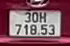
\includegraphics[height=1.7cm]{docs/images/plate_sample_1.png}}{}\hspace{0.8cm}
\IfFileExists{docs/images/plate_sample_2.png}{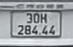
\includegraphics[height=1.7cm]{docs/images/plate_sample_2.png}}{}\hspace{0.8cm}
\IfFileExists{docs/images/plate_sample_3.png}{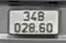
\includegraphics[height=1.7cm]{docs/images/plate_sample_3.png}}{}
\caption{Một số ảnh biển số thực tế được cắt ra và đưa vào mô hình nhận dạng.}
\label{fig:plates}
\end{figure}

Bảng~\ref{tab:samples} đặt cạnh nhau biển số thật và chuỗi mà mô hình đọc được trên một số mẫu trong tập kiểm thử (so sánh sau khi chuẩn hoá). Phần lớn trường hợp mô hình đọc đúng hoàn toàn; mẫu cuối là một ca đọc sai để thấy rõ kiểu lỗi thường gặp.

\begin{table}[H]
\centering
\caption{Ví dụ đầu ra của mô hình trên tập kiểm thử.}
\label{tab:samples}
\begin{tabular}{llll}
\toprule
\textbf{Ảnh} & \textbf{Biển số thật} & \textbf{Mô hình đọc} & \textbf{Kết quả} \\
\midrule
\texttt{car\_104} & 30G58236  & 30G58236  & Đúng \\
\texttt{car\_123} & 89LD00275 & 89LD00275 & Đúng \\
\texttt{car\_130} & 21A08531  & 21A08531  & Đúng \\
\texttt{car\_137} & 30E77379  & 30E77379  & Đúng \\
\texttt{car\_115} & 30F07555  & 30F03055  & Sai \\
\bottomrule
\end{tabular}
\end{table}

Ca sai ở mẫu \texttt{car\_115} là điển hình cho dạng lỗi đã nói ở chương kết quả: mô hình chỉ đọc lệch ở cụm số (đọc \texttt{7555} thành \texttt{3055}), còn phần mã tỉnh và chữ loại xe vẫn đúng. Đây cũng là lý do độ chính xác ký tự cao hơn nhiều so với độ chính xác toàn biển.

\section{Giao diện web kiểm thử (Test Train)}
Để thử mô hình một cách nhanh chóng mà không cần chạy lại toàn bộ pipeline, nhóm xây dựng một trang web kiểm thử (mục \emph{Test Train} trên giao diện, Hình~\ref{fig:webtest}). Người dùng kéo thả hoặc chọn một ảnh, hệ thống sẽ phát hiện biển số bằng YOLO, cắt vùng biển rồi đưa vào mô-đun nhận dạng. Kết quả hiển thị gồm chuỗi biển số đọc được tách theo từng ký tự, mức độ tin cậy, ảnh crop biển số và ảnh gốc, kèm một danh sách lịch sử các lần kiểm thử trước đó. Trang này rất tiện để soi nhanh những trường hợp mô hình đọc sai.

\begin{figure}[H]\centering
\IfFileExists{docs/images/dashboard_detail.png}{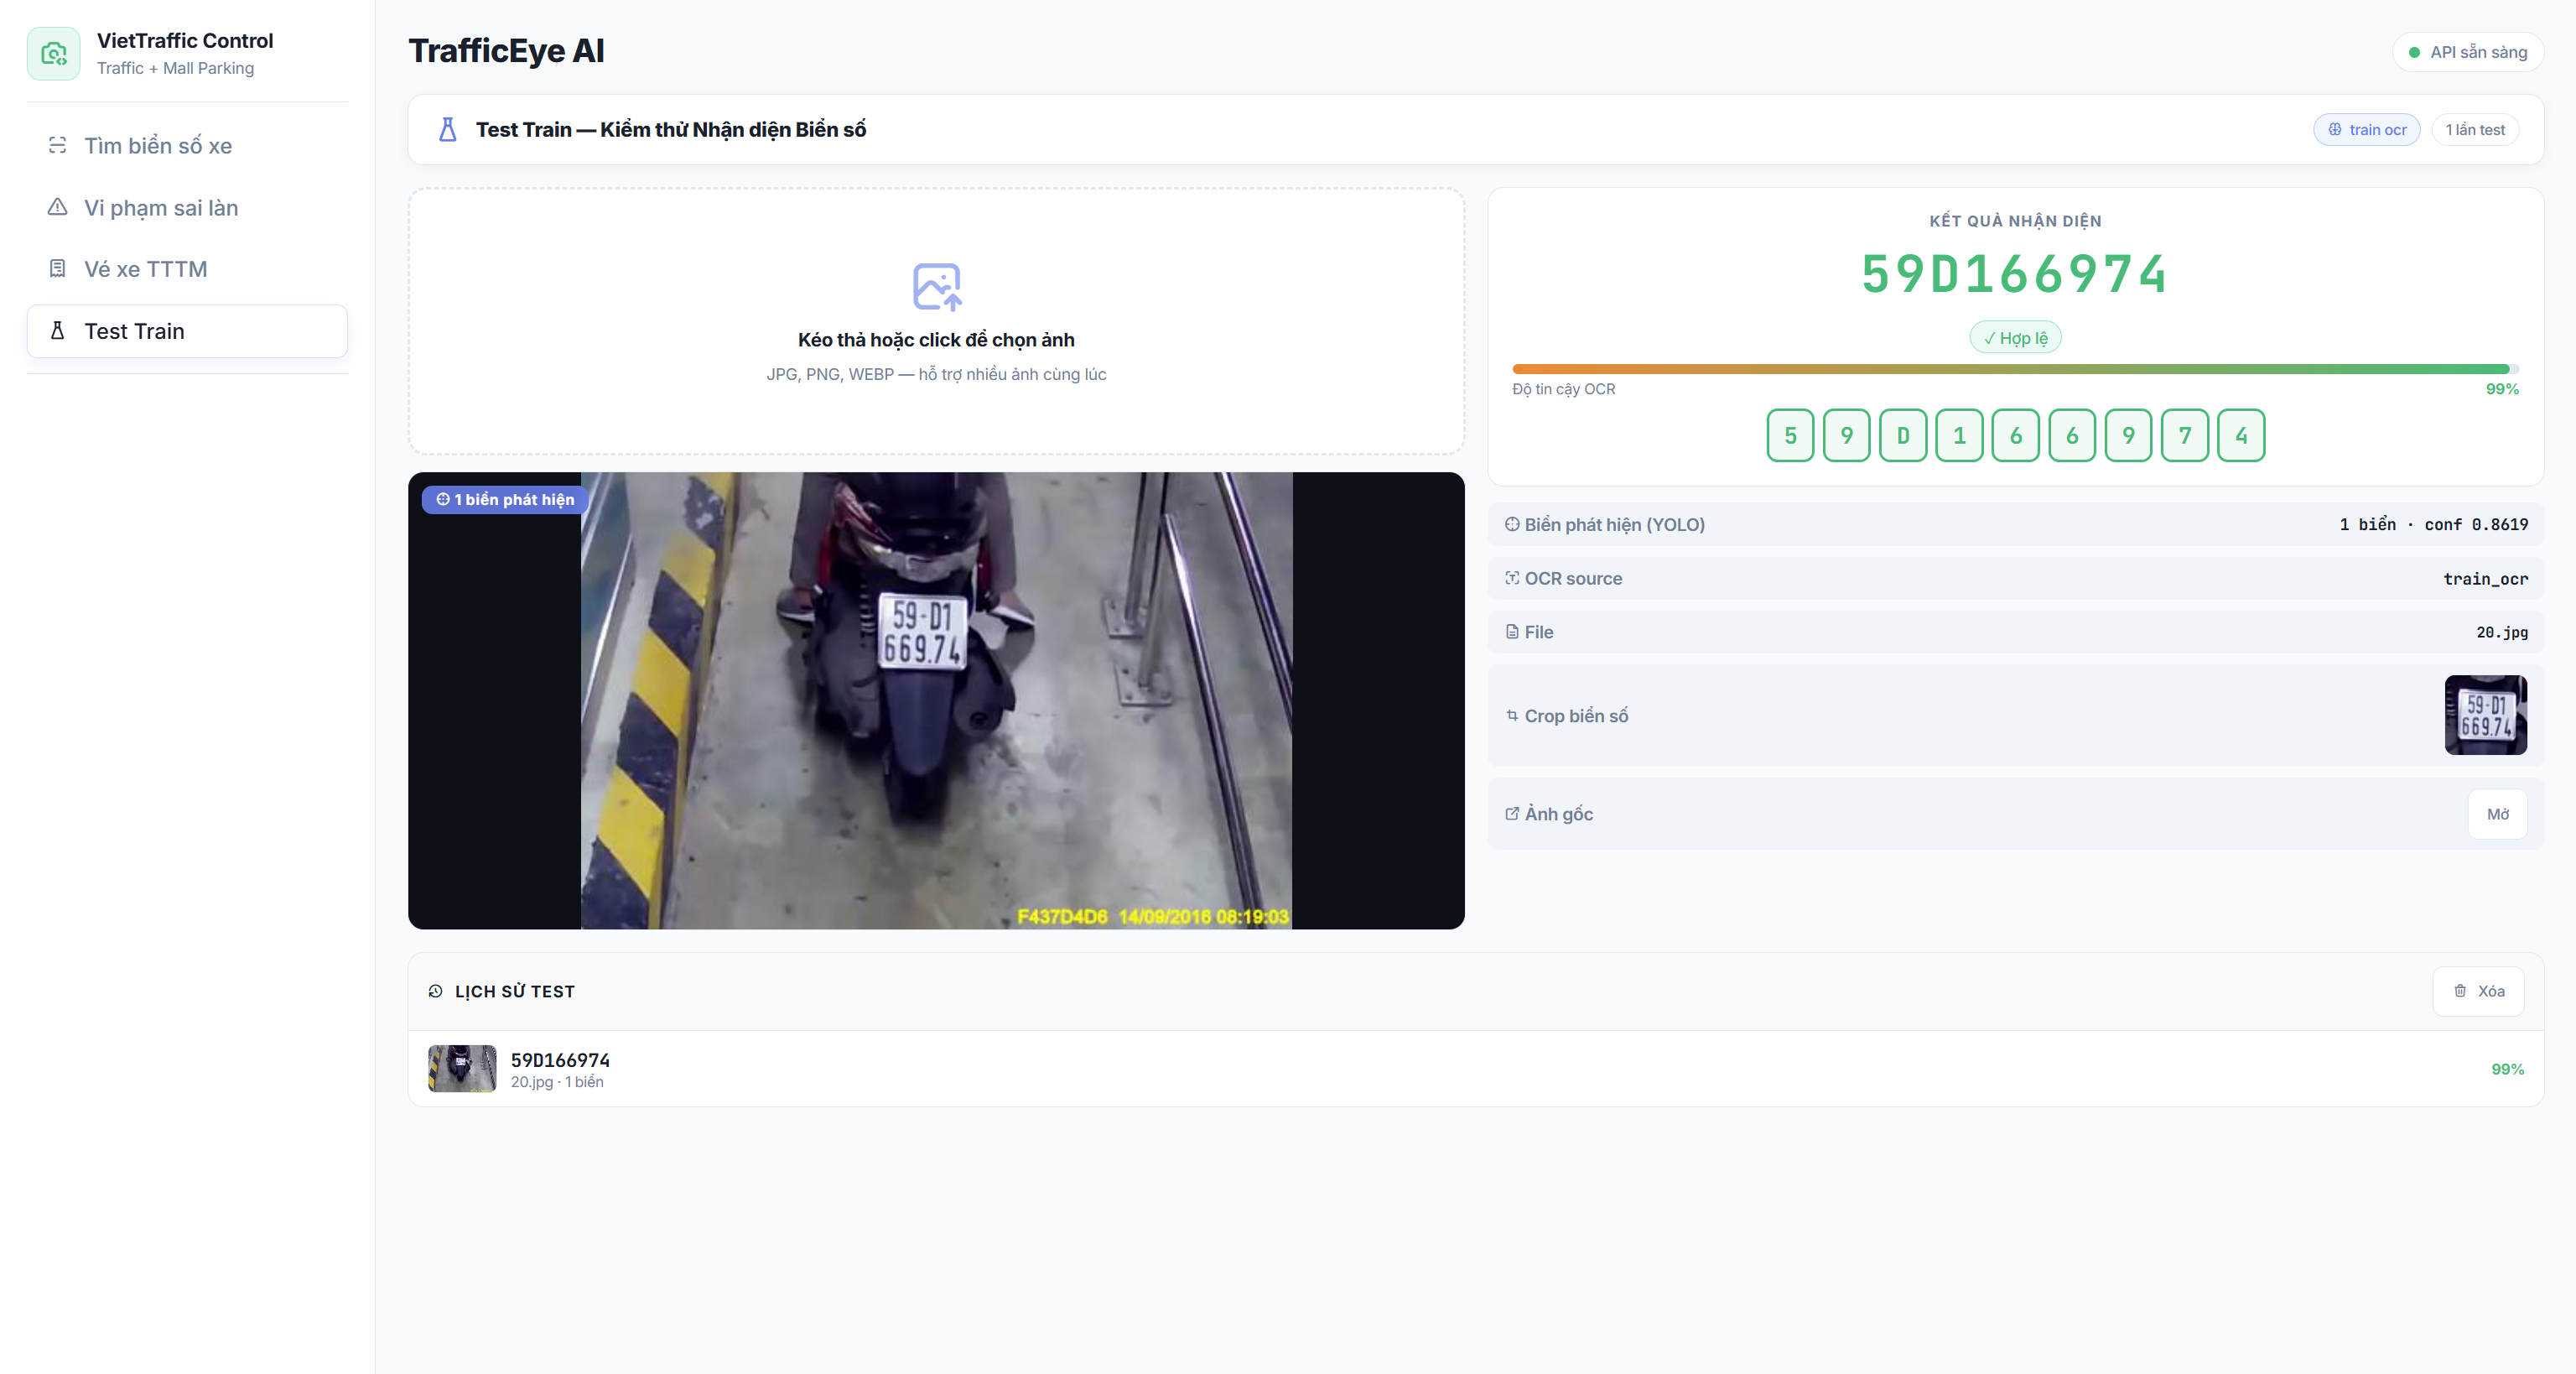
\includegraphics[width=0.92\linewidth]{docs/images/dashboard_detail.png}}{}
\caption{Trang web kiểm thử mô hình (Test Train): tải ảnh lên, phát hiện biển bằng YOLO và hiển thị kết quả nhận dạng theo từng ký tự kèm độ tin cậy.}
\label{fig:webtest}
\end{figure}

\section{Giao diện giám sát và quản trị}
Ngoài trang kiểm thử, hệ thống còn có giao diện vận hành. Màn hình giám sát trực tiếp (Hình~\ref{fig:weblive}) vẽ khung phát hiện phương tiện và biển số ngay trên luồng video. Trang danh sách vi phạm (Hình~\ref{fig:weblist}) tổng hợp các vụ việc đã lưu trong cơ sở dữ liệu, mỗi dòng gồm ảnh bằng chứng, biển số, loại lỗi và mức phạt, thuận tiện cho việc tra cứu và xử lý.

\begin{figure}[H]\centering
\IfFileExists{docs/images/dashboard_live.png}{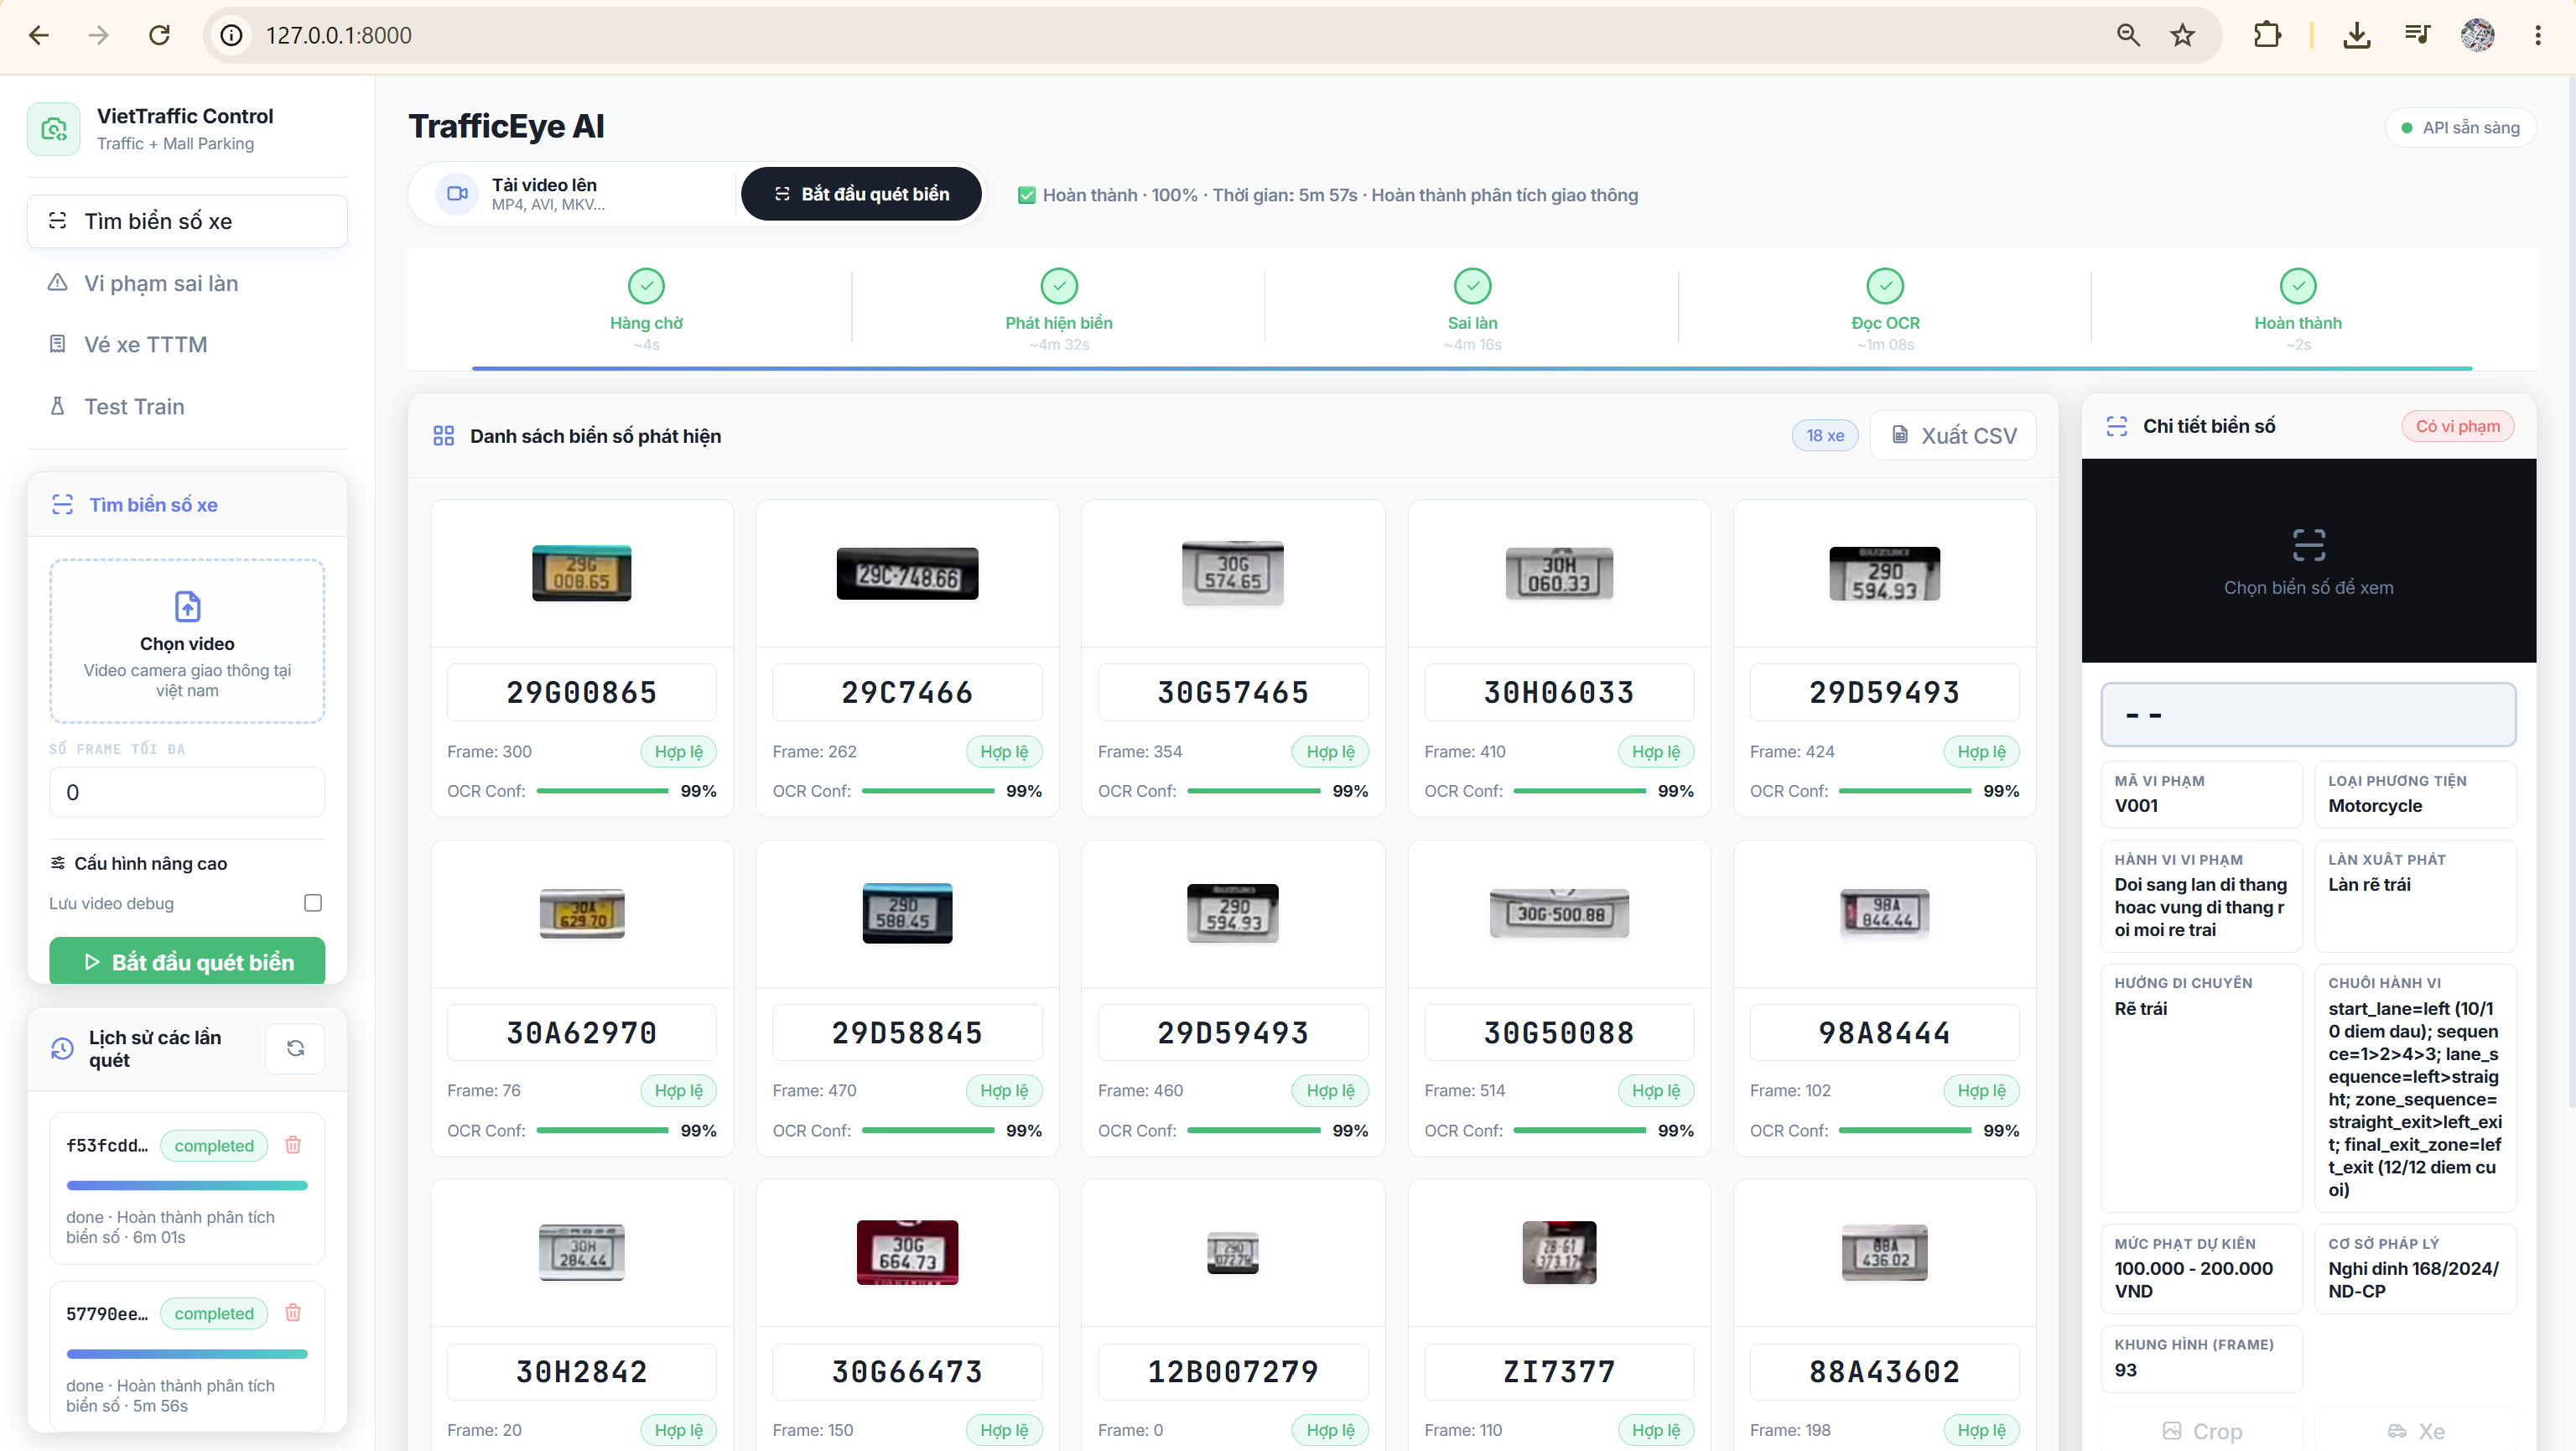
\includegraphics[width=0.92\linewidth]{docs/images/dashboard_live.png}}{}
\caption{Giao diện giám sát trực tiếp trên luồng camera.}
\label{fig:weblive}
\end{figure}

\begin{figure}[H]\centering
\IfFileExists{docs/images/dashboard_list.png}{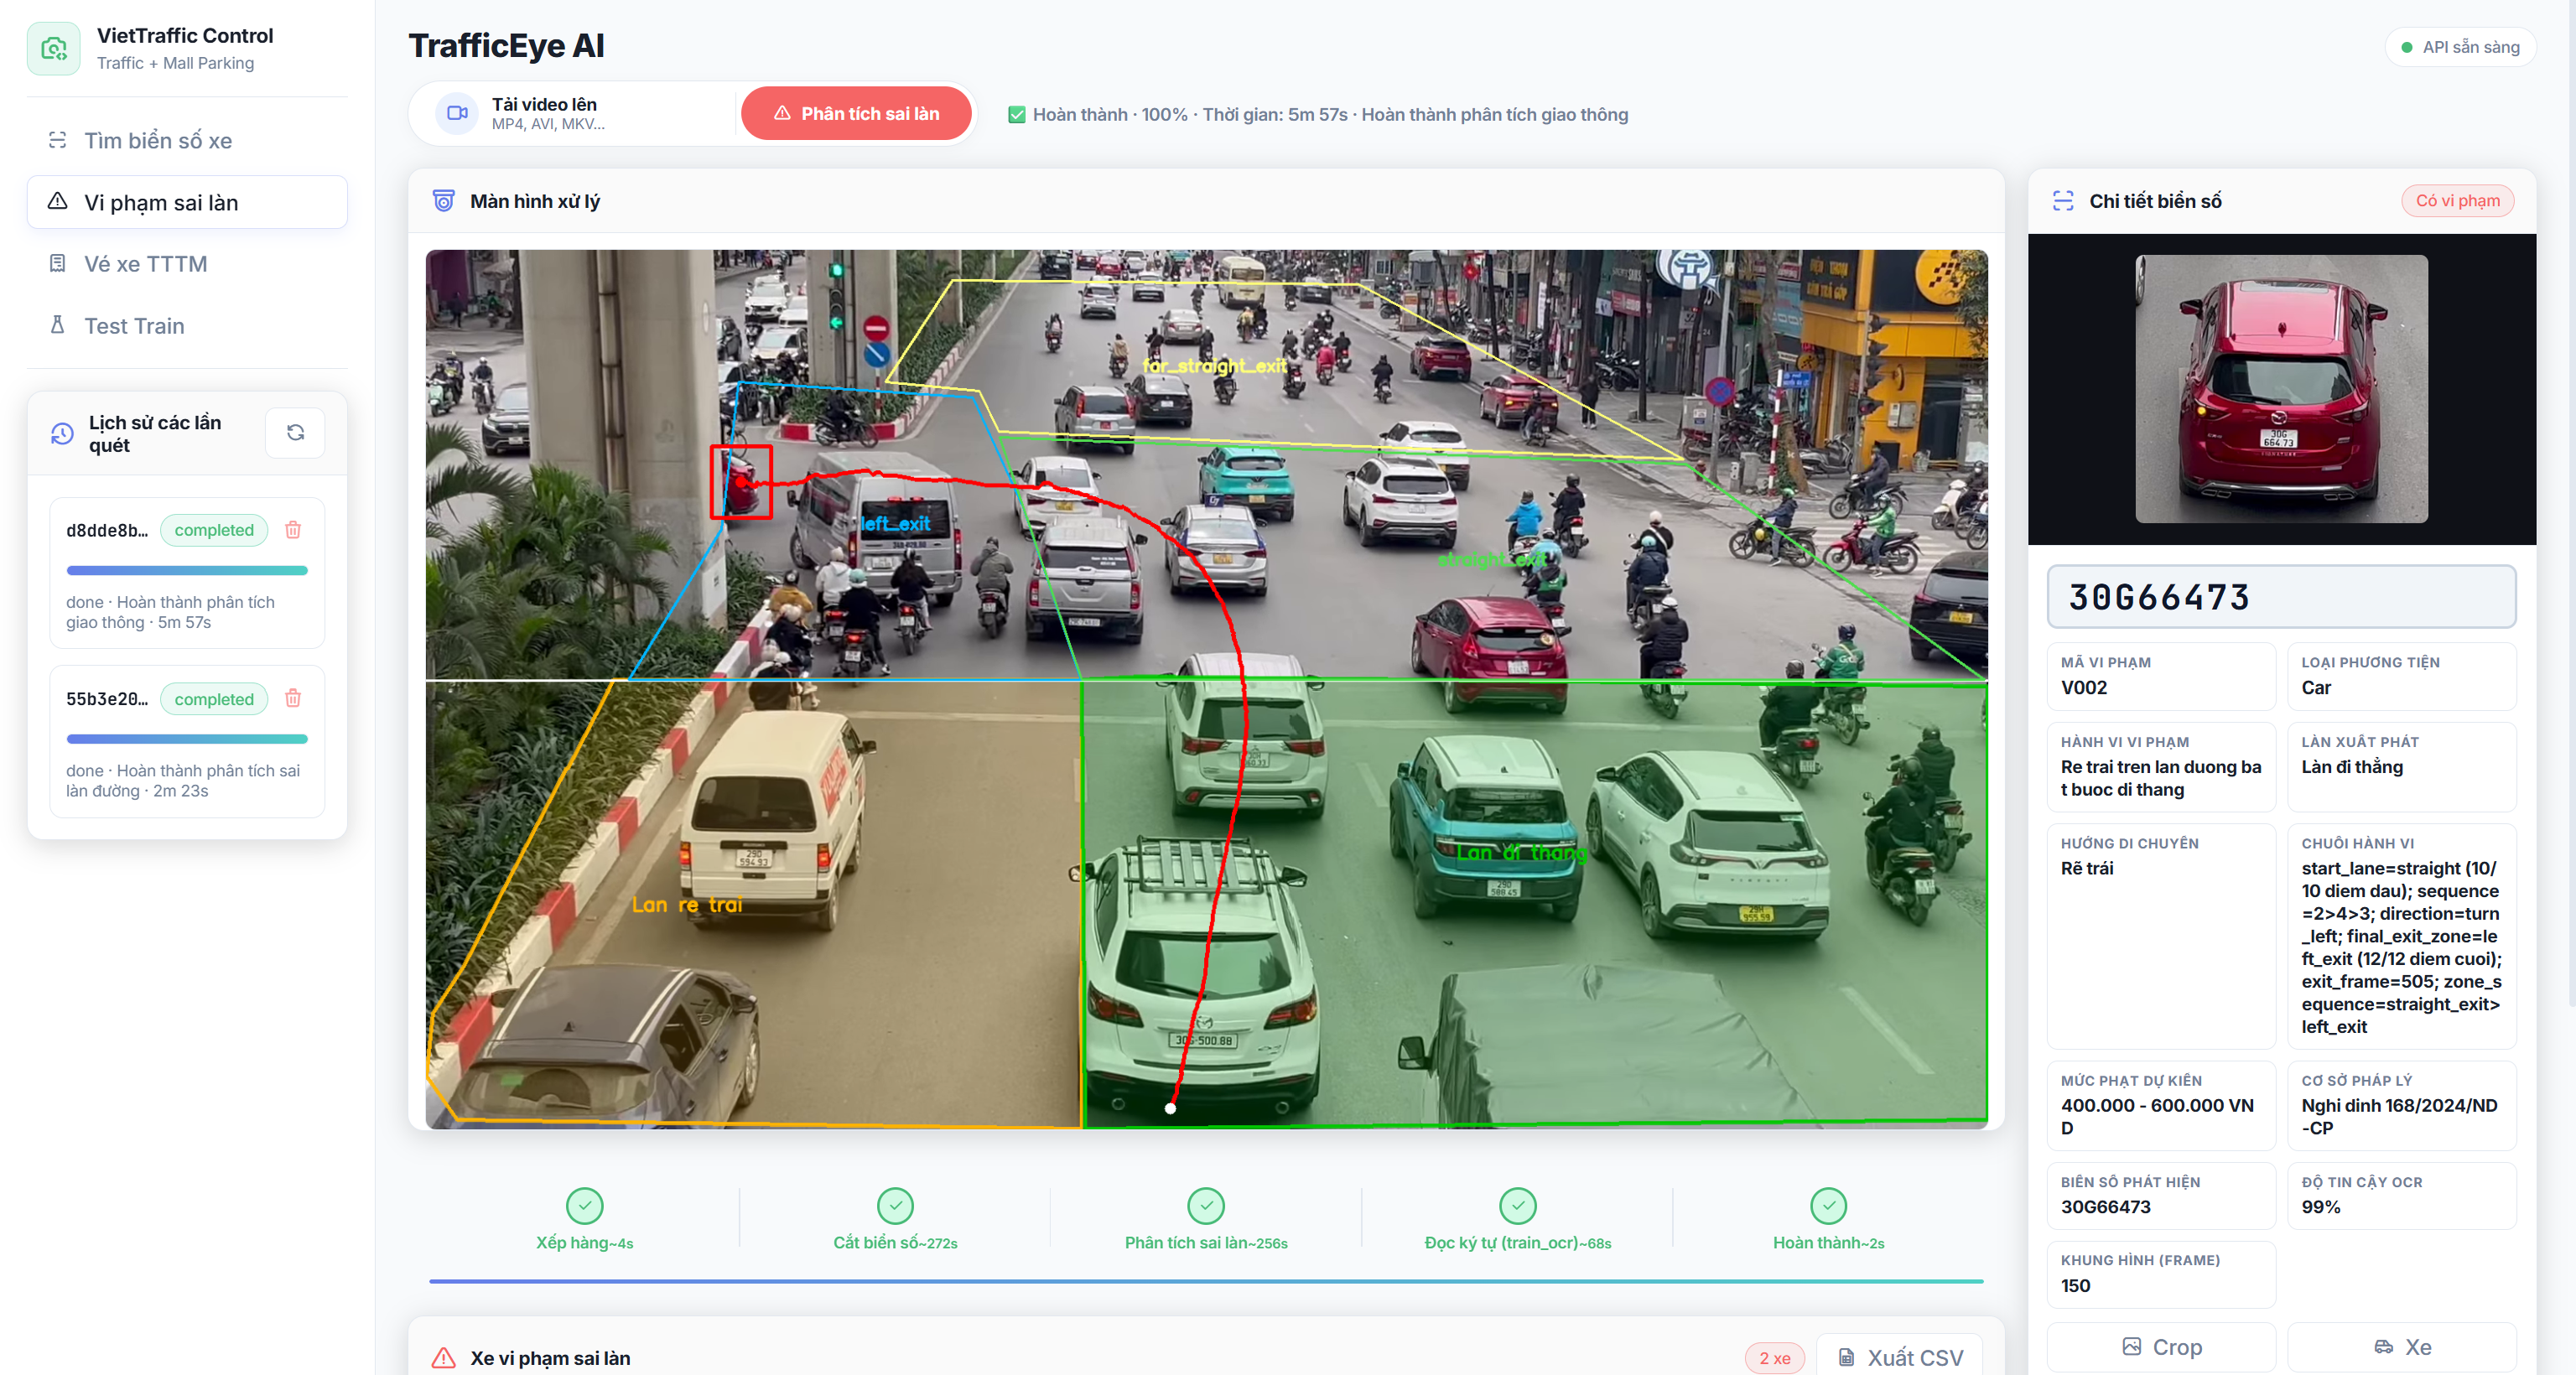
\includegraphics[width=0.92\linewidth]{docs/images/dashboard_list.png}}{}
\caption{Danh sách các vụ vi phạm được lưu trong cơ sở dữ liệu.}
\label{fig:weblist}
\end{figure}

% =====================================================================
\chapter{Phát hiện, bám vết phương tiện và định vị biển số}

Khối nhận dạng ở các chương trước chỉ làm việc tốt khi nhận được một ảnh biển số đủ rõ. Việc tạo ra ảnh đó là nhiệm vụ của khối phát hiện và bám vết phương tiện cùng bộ định vị biển số, đóng vai trò ``tiền xử lý ở mức hệ thống''. Chương này mô tả đúng quy trình mà nhóm đã hiện thực trong mã nguồn (\texttt{find\_license\_plate/main.py}).

\section{Quy trình hoạt động}
Toàn bộ khối vận hành theo một vòng lặp trên từng khung hình, kết hợp với bước chốt kết quả khi mỗi vết kết thúc. Các bước chính như sau:
\begin{enumerate}[leftmargin=*]
  \item Đọc lần lượt từng khung hình của video đầu vào.
  \item Chạy YOLOv8m ở chế độ bám vết (ByteTrack) để phát hiện phương tiện và duy trì \texttt{track\_id}; bỏ qua các phát hiện nằm ngoài vùng quan tâm (ROI).
  \item Với mỗi xe hợp lệ (đã tồn tại đủ số khung tối thiểu và hộp đủ lớn), nới rộng hộp xe $24\%$ rồi chạy bộ phát hiện biển số bên trong vùng đó.
  \item Cắt ảnh biển, đo độ nét bằng phương sai Laplacian và loại bỏ nếu thấp hơn ngưỡng $1800$.
  \item Tính điểm chất lượng cho ảnh biển; nếu cao hơn ứng viên tốt nhất hiện tại của vết và không bị coi là trùng (theo cô-sin, khoảng cách và cửa sổ khung), thì cập nhật ứng viên.
  \item Khi xe rời khung hình hoặc video kết thúc, chốt ảnh biển tốt nhất của vết, chuyển sang khối nhận dạng (OCR) và ghi lại nhật ký theo vết cùng cơ sở dữ liệu.
\end{enumerate}

\begin{figure}[H]
\centering
\begin{tikzpicture}[font=\footnotesize,
  box/.style={draw,thin,fill=white,align=center,text width=8.2cm,minimum height=0.75cm,inner sep=3pt},
  arr/.style={-{Latex[length=2mm]},semithick},node distance=4.5mm]
  \node[box](a){Khung hình video};
  \node[box,below=of a](b){YOLOv8m + ByteTrack: phát hiện và gán \texttt{track\_id}};
  \node[box,below=of b](c){Lọc theo ROI và điều kiện vết hợp lệ};
  \node[box,below=of c](d){Mỗi xe: nới hộp $24\%$ $\rightarrow$ phát hiện biển số};
  \node[box,below=of d](e){Cổng độ nét (Laplacian $\ge 1800$) + tính điểm chất lượng};
  \node[box,below=of e](f){Cập nhật ảnh biển tốt nhất của vết (chống trùng)};
  \node[box,below=of f](g){Vết kết thúc $\rightarrow$ chuyển ảnh biển sang OCR; ghi log \& CSDL};
  \draw[arr](a)--(b);\draw[arr](b)--(c);\draw[arr](c)--(d);\draw[arr](d)--(e);\draw[arr](e)--(f);\draw[arr](f)--(g);
\end{tikzpicture}
\caption{Quy trình hoạt động của khối phát hiện, bám vết phương tiện và định vị biển số.}
\end{figure}


\section{Phát hiện và bám vết phương tiện}
Mỗi khung hình của video được đưa qua bộ phát hiện phương tiện YOLOv8m (\texttt{yolov8m.pt}) với ngưỡng tin cậy $0{,}18$ và ngưỡng IoU $0{,}5$. Để theo dõi cùng một xe qua nhiều khung, hệ thống bật chế độ bám vết của YOLO với thuật toán ByteTrack (tham số \texttt{tracker="bytetrack.yaml"}, \texttt{persist=True}); ByteTrack ghép các phát hiện liên tiếp dựa trên dự đoán chuyển động bằng bộ lọc Kalman và độ trùng IoU, nhờ đó gán cho mỗi xe một mã định danh (\texttt{track\_id}) ổn định.

Không phải vùng nào trong khung hình cũng đáng quan tâm. Hệ thống giới hạn xử lý trong một vùng quan tâm (ROI) có toạ độ tỉ lệ $[0{,}0,\,0{,}40,\,1{,}0,\,1{,}0]$, tức chỉ xét khoảng $60\%$ phía dưới khung hình nơi mặt đường xuất hiện, để loại bớt nhiễu từ phần trên. Một vết chỉ được coi là hợp lệ khi tồn tại đủ tối thiểu bốn khung hình và kích thước hộp xe đủ lớn; điều kiện này lọc bỏ các phát hiện thoáng qua hoặc xe ở quá xa.

\section{Định vị biển số trên từng xe}
Với mỗi xe đang được bám vết, thay vì dò biển số trên toàn khung hình, hệ thống cắt vùng ảnh của xe rồi nới rộng thêm $24\%$ ra bốn phía (để tránh cắt mất ký tự ở mép) và chỉ chạy bộ phát hiện biển số chuyên biệt (\texttt{license\_plate\_detector.pt}, ngưỡng tin cậy $0{,}25$) bên trong vùng này. Cách làm hai bước này vừa thu hẹp không gian tìm kiếm, vừa tăng độ chính xác vì biển số luôn nằm trên thân xe. Mỗi ảnh biển cắt ra được kiểm tra độ sắc nét bằng phương sai của ảnh Laplacian; nếu giá trị này nhỏ hơn ngưỡng $1800$ thì ảnh bị loại vì quá mờ, không đáng tin để đọc.

\section{Chọn khung hình tốt nhất và chống trùng}
Một xe xuất hiện trong nhiều khung với chất lượng khác nhau, nên hệ thống không lấy khung bất kỳ mà chấm điểm từng ảnh biển rồi giữ lại ảnh tốt nhất cho mỗi xe. Điểm chất lượng tổng hợp nhiều tiêu chí:
\begin{equation}
S = 0{,}35\,c + 0{,}25\,\hat{s} + 0{,}20\,\hat{z} + 0{,}10\,\hat{a} + 0{,}10\,\hat{k},
\end{equation}
trong đó $c$ là độ tin cậy của bộ phát hiện, $\hat{s}$ là điểm sắc nét (chuẩn hoá từ phương sai Laplacian), $\hat{z}$ là điểm kích thước biển, $\hat{a}$ là điểm diện tích tương đối và $\hat{k}$ là điểm tương phản. Trọng số dồn nhiều nhất vào độ tin cậy và độ sắc nét, vì đây là hai yếu tố ảnh hưởng trực tiếp tới khả năng đọc đúng của khối nhận dạng.

Để tránh lưu cùng một biển nhiều lần, hệ thống lọc trùng dựa trên ba điều kiện: độ tương đồng cô-sin giữa các ảnh biển từ $0{,}70$ trở lên, khoảng cách giữa hai tâm biển không quá $110$ điểm ảnh, và hai lần xuất hiện cách nhau trong vòng $45$ khung hình. Kết quả cuối cùng của khối này là một ảnh biển số rõ nhất cho mỗi phương tiện, được chuyển sang khối nhận dạng đã trình bày ở các chương trước, đồng thời ghi lại nhật ký theo vết và cơ sở dữ liệu phục vụ truy vết. Cần lưu ý rằng ở chế độ phạt nguội, khối nặng này chỉ được kích hoạt cho những xe đã bị kết luận vi phạm ở chương tiếp theo.

% =====================================================================
\chapter{Phát hiện hành vi đi sai làn}

Khối phát hiện đi sai làn chịu trách nhiệm xác định xe nào vi phạm để kích hoạt việc đọc biển số làm bằng chứng. Ý tưởng tổng quát là dựng lại quỹ đạo của từng xe, đối chiếu với bố cục các làn và vùng hướng được cấu hình sẵn, rồi áp một bộ luật để kết luận. Nội dung dưới đây bám theo mã nguồn \texttt{find\_wrong\_lane/main.py} và tệp cấu hình \texttt{lane\_config.json}.

\section{Quy trình hoạt động}
Khối phát hiện sai làn cũng vận hành theo từng khung hình để dựng quỹ đạo, rồi kết luận khi mỗi vết đã đủ dữ liệu. Các bước chính như sau:
\begin{enumerate}[leftmargin=*]
  \item Nạp cấu hình từ \texttt{lane\_config.json} và dựng các đa giác làn cùng vùng hướng theo kích thước khung hình.
  \item Mỗi khung: chạy YOLOv8m + ByteTrack để phát hiện và bám vết phương tiện, cập nhật chuỗi vị trí (quỹ đạo) của từng \texttt{track\_id}.
  \item Với mỗi điểm trên quỹ đạo, kiểm tra điểm thuộc làn hoặc vùng hướng nào bằng \texttt{cv2.pointPolygonTest} và ghi vào lịch sử vùng của vết.
  \item Khi vết đủ dài, xác định làn xuất phát (làn chứa các điểm đầu) và hướng thực tế (vùng đích ở cửa sổ cuối, kết hợp độ dịch chuyển ngang của quỹ đạo).
  \item Rút gọn chuỗi vùng đã đi qua rồi đối chiếu với bộ luật \texttt{CASE\_3/4/6} cùng các điều kiện giảm oan.
  \item Nếu kết luận vi phạm, chọn khung bằng chứng tốt nhất, xuất ảnh xe và ảnh review, ghi vào \texttt{violations.csv} và cơ sở dữ liệu; ở chế độ tích hợp, kích hoạt khối phát hiện biển số và OCR cho xe này.
\end{enumerate}

\begin{figure}[H]
\centering
\begin{tikzpicture}[font=\footnotesize,
  box/.style={draw,thin,fill=white,align=center,text width=8.6cm,minimum height=0.75cm,inner sep=3pt},
  arr/.style={-{Latex[length=2mm]},semithick},node distance=4.5mm]
  \node[box](a){Nạp \texttt{lane\_config}: đa giác làn + vùng hướng};
  \node[box,below=of a](b){Mỗi khung: YOLOv8m + ByteTrack $\rightarrow$ quỹ đạo theo vết};
  \node[box,below=of b](c){Điểm trong đa giác $\rightarrow$ ghi làn/vùng vào lịch sử};
  \node[box,below=of c](d){Xác định làn xuất phát + hướng thực tế (vùng đích, dx)};
  \node[box,below=of d](e){Đối chiếu luật \texttt{CASE\_3/4/6} + điều kiện giảm oan};
  \node[box,below=of e](f){Vi phạm $\rightarrow$ chọn khung bằng chứng, xuất ảnh + ghi CSDL};
  \draw[arr](a)--(b);\draw[arr](b)--(c);\draw[arr](c)--(d);\draw[arr](d)--(e);\draw[arr](e)--(f);
\end{tikzpicture}
\caption{Quy trình hoạt động của khối phát hiện hành vi đi sai làn.}
\end{figure}


\section{Cấu hình làn đường và vùng hướng}
Mặt đường tại nút giao được mô tả thủ công một lần bằng các đa giác trong \texttt{lane\_config.json}, dùng toạ độ tỉ lệ rồi nhân theo kích thước khung hình ($1920\times1080$). Có hai làn xuất phát: làn \emph{rẽ trái} (cho phép rẽ trái hoặc quay đầu) và làn \emph{đi thẳng} (chỉ cho phép đi thẳng). Bên kia vạch dừng (đặt ở mức $y=0{,}49$) là ba vùng hướng đích giúp suy ra xe thực sự đi đâu: \texttt{left\_exit} (vùng rẽ trái), \texttt{straight\_exit} và \texttt{far\_straight\_exit} (hai vùng đi thẳng gần và xa). Việc tách riêng làn xuất phát và vùng đích cho phép so sánh ``xe ở làn nào'' với ``xe thực sự đi hướng nào''.

\section{Xác định làn xuất phát và hướng di chuyển}
Phương tiện tiếp tục được bám vết bằng YOLOv8m kết hợp ByteTrack như ở chương trước. Với mỗi xe, hệ thống lấy một điểm đại diện và kiểm tra điểm đó thuộc đa giác nào bằng hàm \texttt{cv2.pointPolygonTest} (kiểm tra điểm trong đa giác), từ đó suy ra làn xuất phát. Hướng di chuyển thực tế được xác định theo vùng đích mà xe đi tới ở cuối hành trình: hệ thống xét một cửa sổ cuối gồm khoảng $12$ khung hình và yêu cầu ít nhất ba điểm rơi vào cùng một vùng để kết luận, nhằm tránh nhiễu ở các khung lẻ. Bên cạnh đó, độ dịch chuyển ngang của quỹ đạo cũng được dùng làm dấu hiệu bổ trợ, với các ngưỡng tỉ lệ cho rẽ ($0{,}18$) và đi thẳng ($0{,}10$), cùng một ngưỡng dịch chuyển tối thiểu ($0{,}08$) để bỏ qua các xe gần như đứng yên. Toàn bộ chuỗi vùng mà xe đi qua được rút gọn thành một dãy, ví dụ $1\!\to\!2\!\to\!4\!\to\!3$.

\section{Bộ luật kết luận vi phạm}
Hệ thống chỉ kết luận vi phạm khi hướng thực tế không nằm trong danh sách được phép của làn xuất phát, theo ba trường hợp ở Bảng~\ref{tab:cases}. Để giảm oan, một kết luận chỉ được đưa ra khi xe có làn xuất phát rõ ràng, có đi tới một vùng đích rõ ràng, và hướng thực tế mâu thuẫn với làn; riêng trường hợp \texttt{CASE\_6} còn đòi hỏi xe phải đi qua vùng đi thẳng trước rồi mới kết thúc ở vùng rẽ trái.

\begin{table}[H]
\centering
\caption{Ba trường hợp vi phạm mà hệ thống phát hiện.}
\label{tab:cases}
\begin{tabular}{p{1.6cm}p{2.2cm}p{2.2cm}p{6.0cm}}
\toprule
\textbf{Mã} & \textbf{Làn xuất phát} & \textbf{Hướng thực tế} & \textbf{Kết luận} \\
\midrule
\texttt{CASE\_3} & Làn rẽ trái & Đi thẳng & Đi thẳng trên làn bắt buộc rẽ trái \\
\texttt{CASE\_4} & Làn đi thẳng & Rẽ trái & Rẽ trái trên làn bắt buộc đi thẳng \\
\texttt{CASE\_6} & Làn rẽ trái & Rẽ trái & Lấn sang làn/vùng đi thẳng rồi mới rẽ trái \\
\bottomrule
\end{tabular}
\end{table}

Căn cứ pháp lý ghi trong kết quả là Nghị định 168/2024/NĐ-CP, với tên lỗi ``Không chấp hành hiệu lệnh, chỉ dẫn của biển báo hiệu, vạch kẻ đường''. Mức phạt tham chiếu là $400.000$--$600.000$ đồng đối với ô tô, xe tải, xe khách và $100.000$--$200.000$ đồng đối với xe máy. Ảnh bằng chứng của mỗi xe vi phạm được chọn theo điểm chất lượng kết hợp độ gần camera (kích thước hộp) và độ sắc nét (phương sai Laplacian), để ưu tiên khung rõ nhất thay vì khung cuối.

\section{Kết quả thực nghiệm trên video}
Chạy trên video kiểm thử, hệ thống ghi nhận $141$ vết hợp lệ và kết luận đúng hai trường hợp vi phạm. Trường hợp thứ nhất (V001) là một xe máy (track 296) thuộc \texttt{CASE\_6}: xuất phát từ làn rẽ trái nhưng lấn sang vùng đi thẳng rồi mới rẽ trái, với chuỗi vùng $1\!\to\!2\!\to\!4\!\to\!3$; ảnh rõ nhất được chọn ở khung 93. Trường hợp thứ hai (V002) là một ô tô con (track 456) thuộc \texttt{CASE\_4}: xuất phát từ làn đi thẳng nhưng rẽ trái, với chuỗi vùng $2\!\to\!4\!\to\!3$; ảnh rõ nhất ở khung 150. Mỗi vi phạm được lưu kèm ảnh xe, ảnh review có vẽ đa giác làn và quỹ đạo, một bản ghi trong \texttt{violations.csv} và \texttt{violations.db}, cùng video gỡ lỗi.

\safeimage{docs/images/wrong_lane_review_V001.png}{0.85}{Ảnh review trường hợp V001 (xe máy, \texttt{CASE\_6}): đa giác làn, quỹ đạo và lý do kết luận.}
\safeimage{docs/images/wrong_lane_review_V002.png}{0.85}{Ảnh review trường hợp V002 (ô tô, \texttt{CASE\_4}).}

Khi tích hợp toàn hệ thống ở chế độ phạt nguội, chính hai phương tiện bị kết luận vi phạm này sẽ kích hoạt khối phát hiện biển số và khối nhận dạng đã trình bày trước đó, qua đó hoàn tất một hồ sơ vi phạm gồm lỗi, biển số và ảnh bằng chứng.

% =====================================================================
\chapter{So sánh với hướng phát triển}

Mô hình \emph{train} trình bày ở các chương trước là phương án đã được hiện thực và đưa vào pipeline. Tuy nhiên, trong quá trình làm, nhóm cũng thử nghiệm một hướng đi khác cho khối nhận dạng và xem đó là hướng phát triển tiềm năng. Chương này trình bày ý tưởng của hướng phát triển đó, hai bước cụ thể đã làm, rồi đặt cạnh kết quả của mô hình train để có một cái nhìn cân bằng.

\section{Ý tưởng của hướng phát triển}
Mô hình train dùng bộ mã hoá Transformer, vốn mạnh nhưng ``đói'' dữ liệu khi huấn luyện từ đầu. Hướng phát triển đi theo một lựa chọn khác, đơn giản và tiết kiệm dữ liệu hơn: kiến trúc \textbf{CRNN}, tức kết hợp một thân tích chập (CNN) để rút đặc trưng nét chữ, một mạng hồi tiếp hai chiều (BiLSTM) để học ngữ cảnh chuỗi, và CTC để đọc chuỗi. Lý do chọn CRNN cho bài toán này khá rõ: với biển số là chuỗi ngắn và tập dữ liệu thật không lớn, một mô hình gọn và hội tụ ổn định thường tổng quát hoá tốt hơn một mô hình lớn dễ quá khớp; ngoài ra CRNN có chi phí suy luận thấp, phù hợp khi cần chạy thời gian thực.

Trên nền ý tưởng đó, nhóm thực hiện hai bước nối tiếp nhau. Bước thứ nhất là dựng một mô hình CRNN cơ sở và huấn luyện từ đầu để có một mốc tham chiếu đo được. Bước thứ hai không thay đổi kiến trúc cốt lõi mà chủ yếu \emph{điều chỉnh các tham số huấn luyện} nhằm đẩy độ chính xác lên cao hơn.

\section{Bước 1 --- Mô hình CRNN cơ sở}
Mô hình cơ sở (\texttt{crnn\_base}) dùng thân tích chập kiểu VGG rút gọn, hai lớp BiLSTM rồi một đầu CTC, giải mã theo kiểu tham lam (greedy). Đây là cấu hình CRNN kinh điển, được huấn luyện hoàn toàn từ đầu trên cùng tập dữ liệu. Khi đánh giá trên tập kiểm thử, mô hình đạt độ chính xác toàn chuỗi $83{,}10\%$, độ chính xác ký tự $95{,}68\%$ và tỉ lệ lỗi ký tự (CER) $4{,}32\%$. Cần lưu ý đây là kết quả \emph{thô} của mô hình, giải mã greedy và chưa áp bộ luật định dạng biển số Việt Nam.

\section{Bước 2 --- Điều chỉnh tham số (phiên bản v2)}
Điểm cần nói rõ là phiên bản thứ hai (v2) về bản chất là một đợt \textbf{điều chỉnh tham số} trên chính mô hình CRNN ở bước 1, chứ không phải một kiến trúc hoàn toàn mới. Phần lớn thay đổi nằm ở siêu tham số huấn luyện và một vài cơ chế điều chuẩn nhẹ, được tóm tắt ở Bảng~\ref{tab:v2}. Mục tiêu là giảm quá khớp và cải thiện khả năng phân biệt các chữ số dễ nhầm, từ đó hạ CER.

\begin{table}[H]
\centering
\caption{Một số điều chỉnh tham số chính từ v1 sang v2.}
\label{tab:v2}
\begin{tabular}{p{4.6cm}p{3.0cm}p{3.0cm}}
\toprule
\textbf{Tham số / cơ chế} & \textbf{v1 (cơ sở)} & \textbf{v2 (điều chỉnh)} \\
\midrule
Learning rate & $1{,}5\times10^{-3}$ & $1{,}2\times10^{-3}$ \\
Weight decay & $2\times10^{-4}$ & $5\times10^{-4}$ \\
Warmup & 5 epoch & 8 epoch \\
EMA decay & 0,999 & 0,9995 \\
Chuẩn hoá backbone & GroupNorm & BatchNorm \\
Dropout (neck / head) & 0,25 / 0,15 & 0,30 / 0,20 \\
Label smoothing (CTC) & --- & 0,05 \\
Lấy mẫu cân bằng ký tự hiếm & --- & có (×4) \\
Tăng cường dữ liệu & vừa & mạnh (heavy) \\
SWA / Stochastic depth / SE & --- & có (bổ sung nhẹ) \\
\bottomrule
\end{tabular}
\end{table}

Theo ước lượng trong tài liệu phân tích, các điều chỉnh này có thể giảm CER khoảng $30$--$50\%$ tương đối và tăng độ chính xác toàn chuỗi thêm vài điểm, tức từ mức $\sim$$83\%$ của v1 lên khoảng $93$--$95\%$. Tuy nhiên phải nhấn mạnh: đây là \emph{con số dự kiến theo kế hoạch}, v2 chưa được huấn luyện và đo thực tế, nên chỉ dùng để định hướng chứ không kết luận.

\section{So sánh và nhận định kết quả}
Bảng~\ref{tab:compare} đặt cạnh nhau các phương án. Cột ``Điều kiện'' rất quan trọng, vì các con số không hoàn toàn cùng điều kiện đo.

\begin{table}[H]
\centering
\caption{So sánh mô hình train với hướng phát triển CRNN.}
\label{tab:compare}
\begin{tabular}{p{3.5cm}cccp{3.1cm}}
\toprule
\textbf{Phương án} & \textbf{Seq/Plate Acc} & \textbf{Char Acc} & \textbf{CER} & \textbf{Điều kiện} \\
\midrule
Mô hình train (thô) & 51,31\% & --- & --- & Val, chưa hậu xử lý \\
Mô hình train (toàn pipeline) & 75,39\% & 93,06\% & 6,96\% & Test, đã hậu xử lý luật \\
Hướng 1: CRNN cơ sở & \textbf{83,10\%} & \textbf{95,68\%} & \textbf{4,32\%} & Test, greedy, chưa hậu xử lý \\
Hướng 2: CRNN v2 (điều chỉnh tham số) & 93--95\% (dự kiến) & --- & $\sim$2,2\% (dự kiến) & Kế hoạch, chưa đo \\
\bottomrule
\end{tabular}
\end{table}

Khi đọc bảng, có mấy điểm cần chú ý. Xét riêng năng lực nhận dạng thô trên dữ liệu thật, CRNN cơ sở ($83{,}10\%$) mạnh hơn hẳn mô hình train ở mức thô ($51{,}31\%$); nói cách khác, CRNN đọc đúng nhiều biển hơn ngay từ mạng, còn mô hình train phải dựa nhiều vào hậu xử lý để bù lại. Con số $75{,}39\%$ của train lại là kết quả sau hậu xử lý, nên không thể đặt ngang hàng với $83{,}10\%$ thô của CRNN; nếu áp cùng bộ luật cho CRNN thì nhiều khả năng nó còn cao hơn nữa. Riêng mức $93$--$95\%$ của v2 mới chỉ là dự kiến, chưa đo, nên cũng chưa thể dùng để kết luận hơn thua.

Tóm lại, hướng phát triển CRNN cho thấy tiềm năng vượt mô hình train về độ chính xác nhận dạng thô, và đây là hướng đáng theo đuổi tiếp. Giá trị hiện tại của mô hình train nằm ở chỗ nó đã được hiện thực trọn vẹn và tích hợp vào pipeline đặc thù cho biển số Việt Nam, cùng tốc độ suy luận đạt thời gian thực. Nhìn nhận đúng như vậy sẽ hữu ích hơn cho các bước cải tiến về sau.

% =====================================================================
\chapter{Đánh giá điểm mạnh, điểm yếu và hướng phát triển}

Chương này nhìn lại mô hình \emph{train} một cách tổng thể: nó mạnh ở đâu, còn yếu chỗ nào, vì sao lại như vậy, và nên đi tiếp theo hướng nào. Cách nhìn ở đây là cân nhắc cả mặt được lẫn chưa được, bởi chỉ khi thấy rõ hạn chế mới biết nên cải thiện chỗ nào.

\section{Điểm mạnh}
Trước hết, mô hình được thiết kế đúng bản chất bài toán. Việc tách phần trộn đặc trưng cục bộ bằng tích chập khỏi phần học ngữ cảnh toàn cục bằng Transformer phản ánh đúng cấu trúc của biển số, nơi nét chữ là thông tin cục bộ còn trật tự ký tự là thông tin toàn cục. Cơ chế học đa nhiệm với nhánh ngữ nghĩa phụ trợ là một lựa chọn hợp lý, giúp thân tích chập hội tụ nhanh và ổn định hơn ở giai đoạn đầu.

Mô hình cũng tôn trọng trọn vẹn ba ràng buộc đặt ra: huấn luyện hoàn toàn từ đầu, chỉ dùng dữ liệu được cấp, và chạy trên GPU miễn phí. Điều này đáng ghi nhận về tính tự lực và khả năng tái lập, vì bất kỳ ai cũng có thể dựng lại kết quả mà không cần tài nguyên đặc biệt. Về mặt vận hành, mô hình đạt tốc độ thời gian thực với thông lượng khoảng $13{,}4$ ảnh mỗi giây và độ trễ trung bình quanh $75$ mili-giây cho mỗi ảnh, đủ đáp ứng luồng camera. Cuối cùng, khi đặt trong toàn pipeline, phần hậu xử lý theo định dạng biển số Việt Nam giúp kết quả cuối có cấu trúc hợp lệ, thuận tiện cho mục tiêu làm bằng chứng pháp lý.

\section{Điểm yếu}
Điểm yếu cốt lõi là khoảng cách tổng quát hoá. Độ chính xác trên tập huấn luyện đạt tới $95\%$ trong khi trên tập kiểm chuẩn ở mức thô chỉ còn $51{,}31\%$, cho thấy mô hình quá khớp đáng kể và năng lực nhận dạng thô thực sự còn thấp. Hệ quả là phần lớn độ chính xác cuối cùng (lên $75{,}39\%$) đến từ bước hậu xử lý theo luật chứ không phải từ bản thân mạng nơ-ron; điều này tiềm ẩn rủi ro khi gặp biển ngoài định dạng chuẩn như xe nước ngoài hay biển ngoại giao, lúc đó bộ luật có thể ``sửa nhầm'' và che giấu lỗi thật của mô hình.

Nguồn gốc một phần nằm ở chính kiến trúc: Transformer vốn ``đói'' dữ liệu, trong khi tập thật chỉ khoảng $9{.}700$ ảnh, buộc phải bù bằng tỉ lệ ảnh tổng hợp cao và kéo theo nguy cơ mô hình trôi về đặc trưng tổng hợp. Mô hình cũng còn yếu ở một số phân nhóm cụ thể, rõ nhất là nhóm \texttt{type2} với độ chính xác toàn biển chỉ $54{,}19\%$. Và như đã thấy ở chương so sánh, xét riêng năng lực nhận dạng thô, mô hình hiện chưa vượt được hướng CRNN. Về triển khai, độ trễ $75$ mili-giây tuy đạt thời gian thực trên máy chủ GPU nhưng chưa đủ nhanh cho thiết bị biên như Jetson.

\section{Vì sao kết quả như vậy}
Nhìn tổng thể, nguyên nhân gốc là sự lệch pha giữa độ phức tạp của kiến trúc và quy mô dữ liệu. Một mô hình mạnh như Transformer chỉ phát huy khi có đủ dữ liệu; khi dữ liệu thật hạn chế, nó dễ quá khớp và buộc phải dựa vào dữ liệu tổng hợp cùng hậu xử lý để duy trì kết quả. Trong khi đó, một kiến trúc gọn hơn như CRNN lại tận dụng dữ liệu nhỏ hiệu quả hơn nên cho năng lực thô cao hơn. Bài học rút ra là trong điều kiện dữ liệu hiện tại, độ phức tạp của mô hình không tỉ lệ thuận với độ chính xác, và việc chọn mô hình cần cân nhắc cùng quy mô dữ liệu sẵn có.

\section{Tổng kết và hướng phát triển}
Tổng kết lại, mô hình \emph{train} là một thiết kế bài bản theo hướng hiện đại, được huấn luyện hoàn toàn từ đầu trong ràng buộc tài nguyên chặt và đã chạy được trọn vẹn trong pipeline giám sát, đạt $93{,}06\%$ độ chính xác ký tự và $75{,}39\%$ độ chính xác toàn biển ở tốc độ thời gian thực. Đồng thời, cần thấy rằng đây mới là một kết quả có giá trị tham khảo và còn nhiều dư địa cải thiện, đặc biệt ở năng lực nhận dạng thô.

Trên cơ sở các điểm yếu đã phân tích, nhóm đề xuất một số hướng phát triển tiếp theo:
\begin{enumerate}[leftmargin=*]
  \item Giảm quá khớp bằng cách tăng điều chuẩn, hạ tỉ lệ ảnh tổng hợp và kiểm soát phân phối ảnh tổng hợp sát với ảnh thật hơn.
  \item Nâng năng lực nhận dạng thô, chẳng hạn thêm label smoothing cho CTC, lấy mẫu cân bằng cho ký tự hiếm, hoặc rút gọn số lớp Transformer cho phù hợp quy mô dữ liệu; song song, theo đuổi hướng phát triển CRNN đã trình bày ở chương trước.
  \item Tập trung phân tích và bổ sung dữ liệu cho các nhóm khó như \texttt{type2}.
  \item Tối ưu triển khai bằng cách chuyển sang ONNX/TensorRT và lượng tử hoá để hạ độ trễ xuống mức chạy được trên thiết bị biên.
  \item Đánh giá lại mọi phương án trên cùng một điều kiện đo (cùng tập kiểm thử, cùng có hoặc không có hậu xử lý) để so sánh đúng nghĩa.
\end{enumerate}

\vfill
\begin{center}\small\itshape
Các số liệu trong báo cáo đều được ghi kèm điều kiện đo thực tế của dự án, với phần thô và phần toàn pipeline tách bạch rõ ràng để người đọc tiện đối chiếu.
\end{center}

\end{document}
